\documentclass[11pt,a4paper,twoside,twocolumn]{article}
%\documentclass[11pt,a4paper]{article}
\usepackage{graphicx,parskip,times,amsfonts,amsmath,url}
%\usepackage{esc-handbook-org}
%\usepackage{eurosym}
%\usepackage{natbib}
\usepackage{a4,a4wide}
%\usepackage[german]{babel}
\usepackage{amssymb,amsmath,amsfonts}
\usepackage[today]{../../../lib/macros/svninfo}
\usepackage[show]{ed}
%\includeonly{kohlhase,schoenwaelder}
\def\shorttitle#1{}
%---------------------PDF-definitions--------------------------------------
\usepackage[pdftex,           %%% hyper-references for pdflatex
  hypertexnames=false,%       %%% needed for correct links to figures
  breaklinks=true,%           %%% break links if exceeding a single line
  colorlinks=true,%           %%% to underline links instead of boxing
  urlcolor=blue]{hyperref}    %%% blue instead of cyan URLS
%---------------------end-of-PDF-definitions-------------------------------

\newcommand{\mycaption}[1]{\caption{{\sl #1}}}
\renewcommand*{\cleardoublepage}{\clearpage\if@twoside \ifodd\c@page\else
    \hbox{}
    \if!\blankpagetext!\else
    \vfil \begin{center} \setlength{\fboxsep}{3mm}%
    \framebox{\blankpagetext}
    \end{center}\vfil\vfil \fi
    \newpage\if@twocolumn\hbox{}\newpage\fi\fi\fi}
\newcommand*{\resetpages}{\cleardoublepage\pagenumbering{arabic}}
\raggedbottom \pagenumbering{Roman}
\renewcommand{\labelitemi}{-}

\newenvironment{myitemize}{\begin{list}{-}{\labelwidth=0.2cm \leftmargin0.4cm
\labelsep0.2cm \rightmargin0cm \parsep0.5ex plus0.2ex minus0.1ex
\itemsep0ex
 plus0.2ex}}{\end{list}}

\setlength{\parskip}{0pt plus 1pt}

\title{SES Research Area 1\\
  Information and Communication Technologies}
\author{}

\begin{document}
\maketitle
\svnInfo $Id: report.tex 1229 2006-11-20 17:13:48Z birk $
\svnKeyword $HeadURL: https://subversion.eecs.iu-bremen.de/svn/eecs/eecs/research-report/2006/report.tex $
\begin{center}
  \begin{tabular}{|l|l|}\hline
    {\bf{Source Information}} & 
    revision \svnInfoMaxRevision, last change {\svnInfoLongDate} 
    \def\empty{}\ifx\svnInfoOwner\empty\else by {\svnInfoOwner}\fi\\\hline
    \multicolumn{2}{|l|}{{\scriptsize\tt{\svnInfoHeadURL}}}\\\hline
  \end{tabular}
\end{center}

\shorttitle{Information and Communication Technologies}
\section{Information and Communication Technologies}

The increasing impact of information and communication technology dominates our everyday
life, our society, and the environment.  Examples comprise the World-Wide-Web, the
ubiquitous use of computers, cellular multimedia and wireless communications, robots in
factories as well as in offices and homes, and sophisticated computer models used to
predict the evolution of complex systems such as the global climate.

The enormous level of integration in micro-electronics has enabled unprecedented progress
in many sectors -- and even more importantly, it has created many new profitable
technologies and services based on them. The 21st century will witness technologies that
enable machines to do things that have been so far restricted to humans: machines will be
able to sense, act, speak, listen, decide and sometimes understand. Our T-shirts may have
their own Internet addresses and wirelessly tell the laundry machine about proper
treatment. We will see cars that negotiate with each other in order to maximize traffic
flow while reducing pollution using sophisticated energy management systems. Manufacturing
technologies will improve using a combination of detectors and software to control
processes. Robots are also more and more used in domains where some autonomy and
intelligence is necessary. They work under conditions where it is unpleasant or even risky
for humans like in abandoned mines or at disaster sites and where they have to deal with
situations unforeseen by their designers and programmers. The hallmark of such smart
systems is their integration of technologies from analogue devices and sensors,
communication systems and networks, internet services, artificial intelligence, machine
learning, robotics, and many more.

The School of Engineering and Science actively contributes to this
rapidly growing, boldly interdisciplinary endeavor, focusing on the
areas described in the following.
%
%{\em{Mathematical and Symbolic Modeling}\\
%  \item Reasoning and Semantics
%  \item Simulation and Control of Complex Systems
%  \item Machine Learning
%  \end{itemize}
%\item {\em{Communication Networks and Systems}}, in particular:
%  \begin{itemize}
%  \item Wireless and Cellular Communications
%  \item Digital Transmission Methods and Coding
%  \item Networks and Protocols
%  \item Harmonic Analysis applied to communications engineering
%  \end{itemize}
%\item {\em{Robotics and Embedded Systems}}, in particular:
%  \begin{itemize}
%  \item Robotics
%  \item Applied Algorithms
%  \end{itemize}
%\item {\em{Knowledge and Information Management Systems}}, in
%  particular:
%  \begin{itemize}
%  \item Raster Data Services
%  \item Knowledge Management Systems
%  \item Distributed Systems
%  \item Hierarchical Data Representation
%  \end{itemize}
%\item {\em{Microelectronic Devices and Technologies}}, in particular:
%  \begin{itemize}
%  \item Electronic Devices and Nano Photonics
%  \item Microelectronics
%  \end{itemize}
%\item {\em{Digital Signal Processing}}, in particular:
%  \begin{itemize}
%  \item Signal Processing in Communications
%  \item Nonlinear Signal Processing and Control
%  \end{itemize}
%\end{enumerate}

%%% Local Variables:
%%% mode: latex
%%% TeX-master: "report"
%%% End:

\shorttitle{Communication Networks and Systems}
\subsection{Communication Networks and Systems}

The basic desire of modern society to be able to access and
distribute ``any'' information at ``anytime'' and ``anywhere'' is
the driving force for the rapid development of communication
networks and systems. The implications of these goals are manifold
and require truly interdisciplinary research efforts. A typical, but
clearly not complete, list of involved high level research fields
includes

\begin{myitemize}
\item Wireless Network Engineering and System Design
\item Network Interoperability
\item System capacity management and optimization
\item Information transmission
\item Network protocols 
\item Information security.
\end{myitemize}

All these research areas are strongly inter-related and the strength
of a research cluster in ``communication networks and systems''
resides in the close cooperation of the respected research groups
involved. The particular `flat hierarchy' at IUB (no departments and
chairs) fosters such cooperations.

%%% Local Variables:
%%% mode: stex
%%% TeX-master: "report"
%%% End:


\subsubsection{Cellular and Wireless Communications}
\label{Haas1} \index{Haas, Harald}

\paragraph{Research Team}
Harald Haas (Professor), Rami Abu-Alhiga (PhD Student), Zubin
Bharucha (PhD Student), Hany Elgala (PhD Student), Ellina Foutekova
(PhD Student), Birendra Ghimire (PhD Student), Dennis Kolyuzhnov
(PhD Student),  Raed Youself Mesleh (PhD Student), Abdurazak Mudesir
(PhD Student), Hrishikesh Venkataraman (PhD Student), Sinan
Sinanovic (Research Associate), Peter Omiyi (Postdoc), Mostafa
Afgani (Research Engineer), Sudharasan Ganesan (Graduate Student)\\

Research in Cellular and Wireless Communications is geared towards
new technologies. Particular focus is  on the development and the
interaction of key air-interface building blocks \newpage

\begin{myitemize}
\item multicarrier transmission (in particular OFDM (Orthogonal Frequency Division
Multiplexing)
\item duplexing techniques (in particular time division duplexing
(TDD))
\item multiple-input multiple-output (MIMO) techniques
\item wireless ad hoc systems
\item medium access control (MAC) algorithms
\item multiple access and scheduling techniques
\item dynamic channel assignment (DCA) algorithms
\item mobile positioning
\item visible light communication.
\end{myitemize}

\myparagraph{Highlights} \emph{Spatial Modulation.} Spatial
modulation (SM) is a new and patented multiple antenna transmission
approach for wireless systems that increases the spectral efficiency
(number of bits transmitted per Hz bandwidth) by utilizing the
transmit antenna number as an implicit source of information. A
block of information bits is mapped to an information symbol and a
transmit antenna number. As a consequence, at any given time instant
only a single antenna of the antenna array is transmitting signal
power. The actual block of information bits determines which antenna
is active at a particular time instant. As a result, inter-channel
interference (ICI) at the receiver input and the need to synchronize
the transmit antennas are completely avoided. Simple receiver
algorithms such as maximum receive ratio combining (MRRC) can be
used to retrieve the information bits. The performance and the
receiver complexity of SM and V-BLAST (Vertical-Bell Labs Layered
Space-Time) algorithm in flat fading channels are compared. V-BLAST
applies zero forcing detection based optimum ordering, nulling and
successive interference cancellation. The basic principle of SM is
depicted in Fig.~\ref{smexmpl}, and results of the comparison with
state-of-the-art V-BLAST are shown in Fig.~\ref{fig55}.
\begin{figure}[!htb]\centering
  \centerline{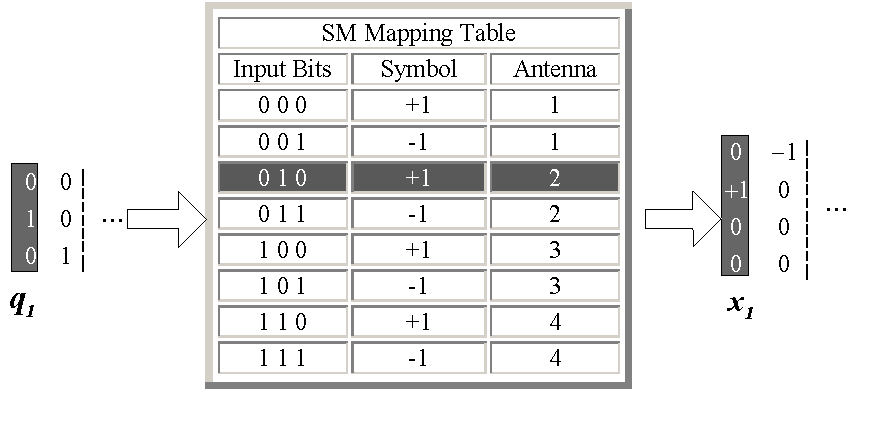
\includegraphics[width=8cm]{haas_1.pdf}}
  \caption{3bits/symbol spatial modulation mapping table using binary phase shift keying (BPSK)
    and four transmit antennas} \label{smexmpl}
\end{figure}
\begin{figure}[!!htp]\centering
  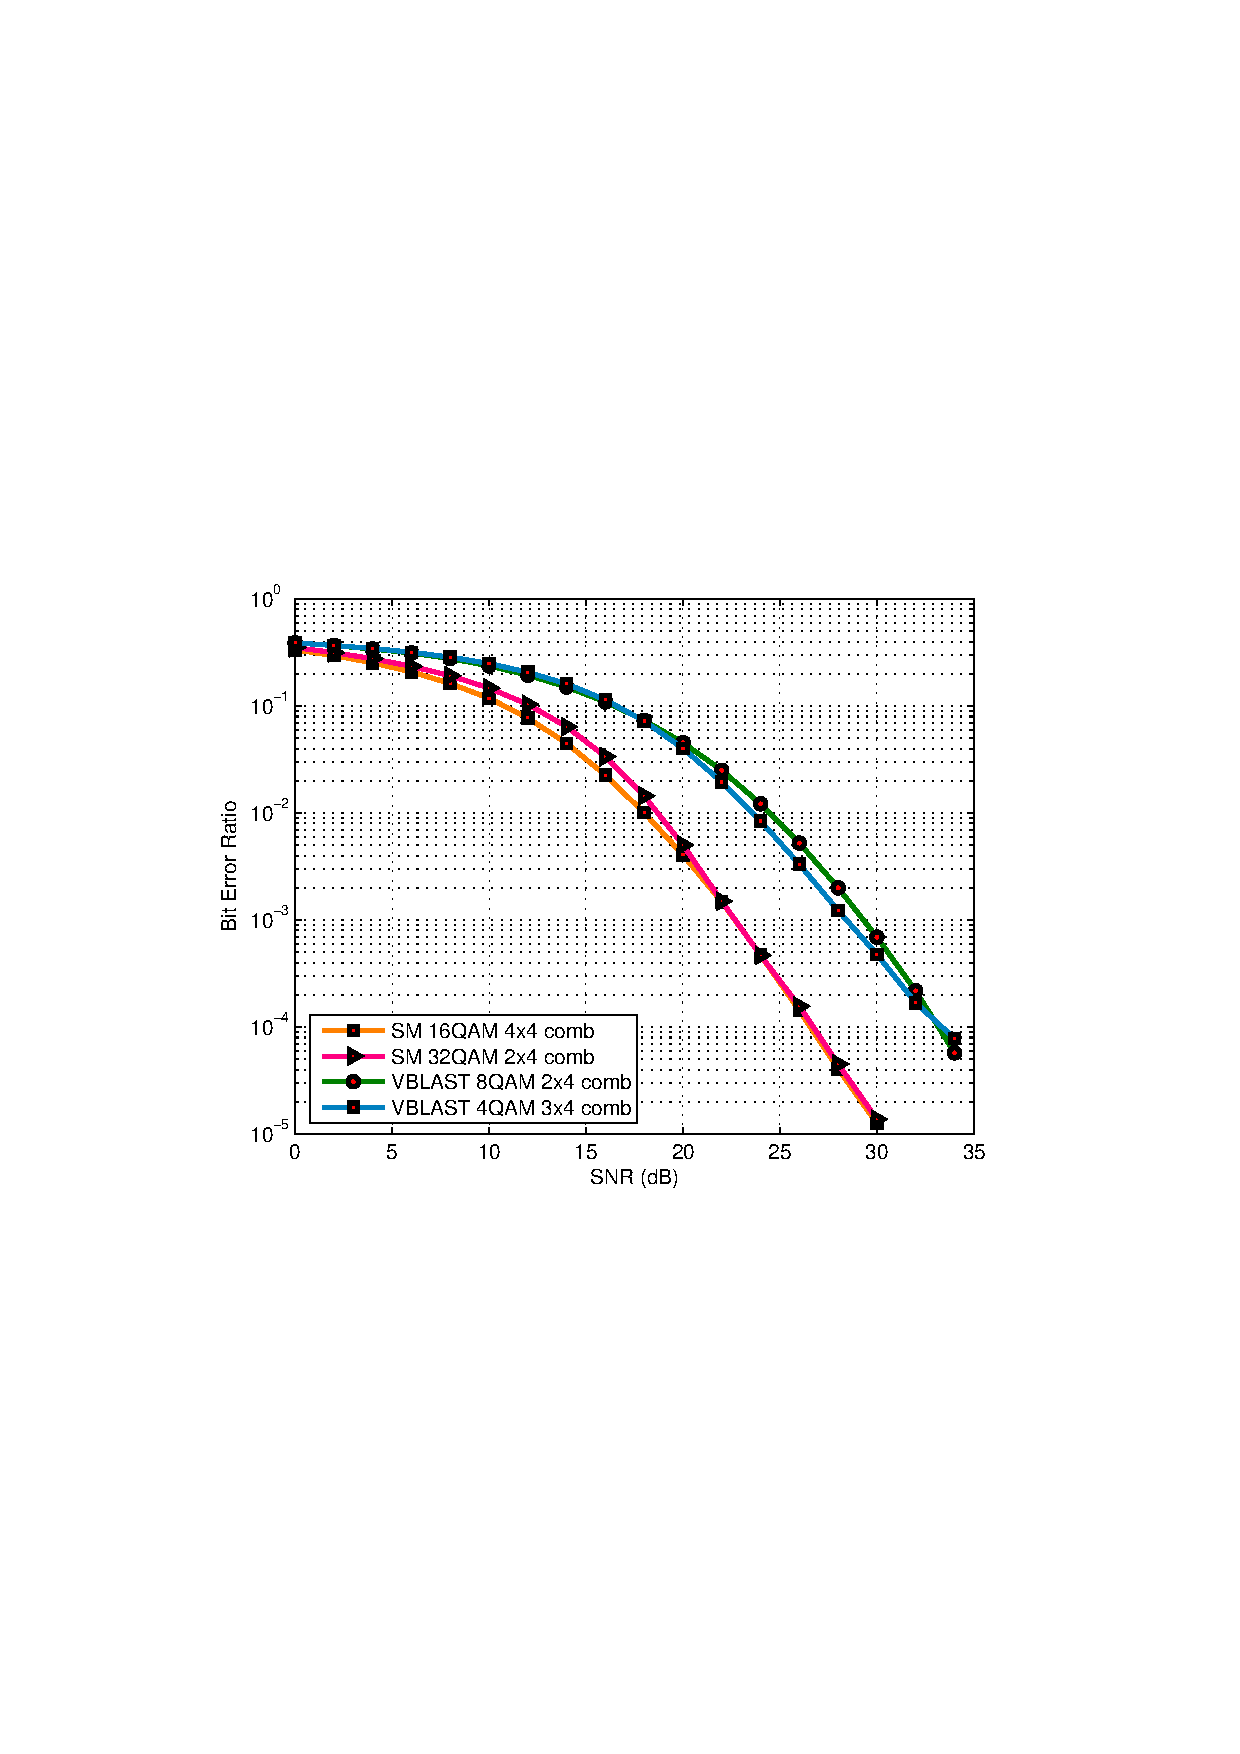
\includegraphics[width=8cm]{haas_2.pdf}\\
  \caption{Bit error performance as a function of signal-to-noise ratio (SNR) for state-of-the-art V-BLAST and novel SM.}
  \label{fig55}
\end{figure}
From the results it can be found that the performance gains are
significant. In both schemes the same number of bit per unit
bandwidth are transmitted (for fair comparison), but with SM the bit
error performance is reduced considerably. For example, at an SNR of
20dB a 10-fold reduction in the BER is observed.

\emph{Dynamic Resource Allocation.} In this work a fully
decentralized interference avoidance algorithm to manage
interference in an \emph{ad hoc} wireless network, applicable to
wireless sensor networks, is developed and analyzed. Fig.~\ref{dca}
depicts a randomly chosen distribution of transmitting (Tx) and
receiving (Rx) nodes. The new algorithm, called \emph{busy tone
interference tolerance signaling}, is of low complexity and is very
easy to implement. It is based on different functions to set the
busy tone signal power dependent on the level of tolerable
interference, and their performance is compared with a special case
of a fixed power system which provides maximum capacity assuming
equal transmit powers. Results show that an appropriately chosen
function for setting the busy-tone can lead to gains in capacity
using very little power. This power efficiency advantage is quite
significant, implying that battery life of units can be extended
while providing a similar capacity than a fixed power system.
\begin{figure}[!!htp]
 \centering
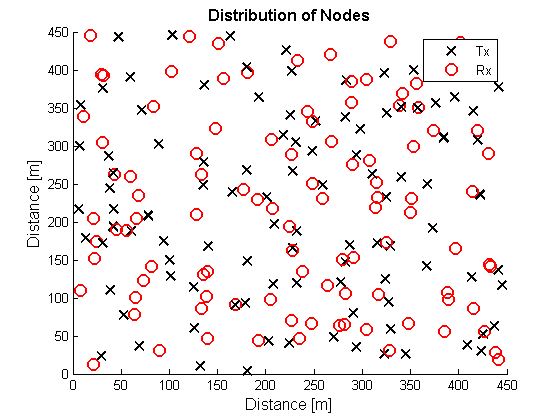
\includegraphics[width=8cm]{haas_3.png}\\
\caption{Random distribution of nodes in an \emph{ad hoc} wireless network}
\label{dca}
\end{figure}

%\null Harald Haas is also involved in ``Signal Processing''
%(Section~\ref{Haas1}).

%\newpage
\paragraph{Organization}
% list the (research) events you have organized, if any,
\begin{enumerate}
    \item Member of Technical Program Committee of and session chair
          at \emph{IEEE International Conference on Personal, Indoor \& Mobile Radio Communications} -- PIMRC 2006
    \item Member of Technical Program Committee of \emph{International IEEE Conference on Vehicular Technology} -- VTC 2006
\end{enumerate}

\paragraph{Collaborations}
\begin{enumerate}
\item {\sl The University of Edinburgh, UK}\\
  Prof. S. McLaughlin\\
  Joint project with industrial partner on \emph{Hybrid Cellular and Multihop Wireless
    Networks}
\end{enumerate}

\newpage
\paragraph{Grants}
% list the running grants in 2005, if none have been received, please delete this
% subsection.
\begin{enumerate}
    \item Funded by industry partner,
      \emph{Cellular TDD-OFDM (Time division duplex - orthogonal frequency
          division multiplexing)},  June 2004 - July 2005


    \item Funding by industry partner and University of Edinburgh, \emph{Hybrid Cellular and Multihop Wireless
    Networks},  July 2005 - July 2006

    \item Funded by industry partner, \emph{Link Adaptation and Scheduling in Cellular
    Systems},  March 2005 - February 2008

    \item Funded by Bremen T.I.M.E program funded by BIS
    Bremerhaven, \emph{Mobile Positioning (MPos)} in collaboration with MobilTec GmbH and supported by
     T-Mobile,  June 2006 - September 2009

    \item Funded by DFG Schwerpunktprogram TakeOFDM, \emph{DCA Algorithms and MAC Protocols for COFDM Based Cellular and
     Ad hoc Systems Using Carrier Sensing Time Division Multiple Access
     (CSTDMA)},  October 2004 - September 2006

\end{enumerate}

\paragraph{Patents}
% list the grants you have received in 2005, if none have been received, please delete this
% subsection.
\begin{enumerate}
\item Four new patent applications submitted
\item Three previously submitted patents got granted in 2006
\end{enumerate}

\paragraph{Awards, Prizes}
\begin{enumerate}
\item Nominated for the Chinese 111 Program -- Guest Academic Talents Programme for the Development of University Disciplines in China
\item Invited Talk at the University of Mondragon (Spain)
%    \item Honorary Fellowship of Edinburgh University
%    \item Invited to Institute for Digital Communications (IDCOM) at the University of
%          Edinburgh on \emph{Vodafone Fellowship on Communications}
    %\item Invited speaker at \emph{International Next Generation Wireless Network Workshop},
     %     Edinburgh/Scotland
\end{enumerate}

%\paragraph{Publications}
% list the publications of 2005 (also accepted and in press), if none have been received, please delete this
% subsection. Enter the publications into the SES publications database at
% http://kwarc.eecs.iu-bremen.de/ses-pubs/index.php and only reference them here.

 
\nocite{ah06_vis_light}
\nocite{bh06_ped_dead_reck}
\nocite{hnona06_iamac}
\nocite{vh06_thru_cap}
\nocite{cvh06_freq_syn}
\nocite{feh06_semi_analytic}
\nocite{fagvh06_sch_CDMA}
\nocite{jhm06_adhoc_tdd_underlay}
\nocite{oha06_tsalloc_insotdd}
\nocite{mhay06_spatialmod}
\nocite{asilomar06}
\nocite{chinacom06}
\nocite{tdd_book}
\nocite{oha07}
 

 
\subsubsection{Digital Transmission Methods and Coding}
\label{ict:cns:henkel} \index{Henkel, Werner}

\paragraph{Research Team}
Werner Henkel (Professor), Fangning Hu (PhD Student), Neele von Deetzen (PhD
Student), Khaled Shawky Hassan (PhD Student), Apirath Limmanee (PhD Student)\\

We currently concentrate on iterative decoding and unequal error protection in
coding and physical transport. In iterative decoding, we study the convergence
behavior and properties of analog Turbo-like codes and the possible design of
Turbo and LDPC codes for unequal error protection (UEP). In the design of UEP
codes, we especially cooperate with ENSEA, France, and Lule\aa\ University,
Sweden. UEP is also the goal in our multicarrier research, where we design
bit-allocation algorithms that allow for easy realization of different
protection classes in an arbitrary way. UEP will be a must for current and
especially future triple-play data services to different devices at varying
channel qualities.

The analog codes have a strong relation to signal processing. Regarding
practical applications of such codes, we especially look into the correction
of impulse-noise and clipping effects. There, the most important task is to
determine statistical properties that allow for easy erasure marking, which
would support further decoding steps, analog and digital.

We further started a project on data transmission using ultrasound signals. We
currently design lab experiments to deliver data for later modeling of the
channel and disturbances.

%%% give a very short (150 words description of your research area)
%% Hint: this can be copied from the research areas document (../masterplan/research-areas)

\paragraph{Highlights}

The design of UEP Turbo codes by a pruning approach led us to a structure that
we named hybrid concatenation, a combination of outer parallel and inner
serial concatenation. The study of the decoding convergence with so-called EXIT
charts yielded the result that the area between the curves describing the
outer iterations depend on the number of inner iterations. This allows for
minimizing the decoding complexity by a scheduling with varying number of
iterations in the different decoding steps (see Fig.~\ref{fig:henkel_1}). The
pruning concept was also the starting point for our design of UEP LDPC codes
with an irregular check-node profile (pat. pending).

\begin{figure}[ht]
  \centering
  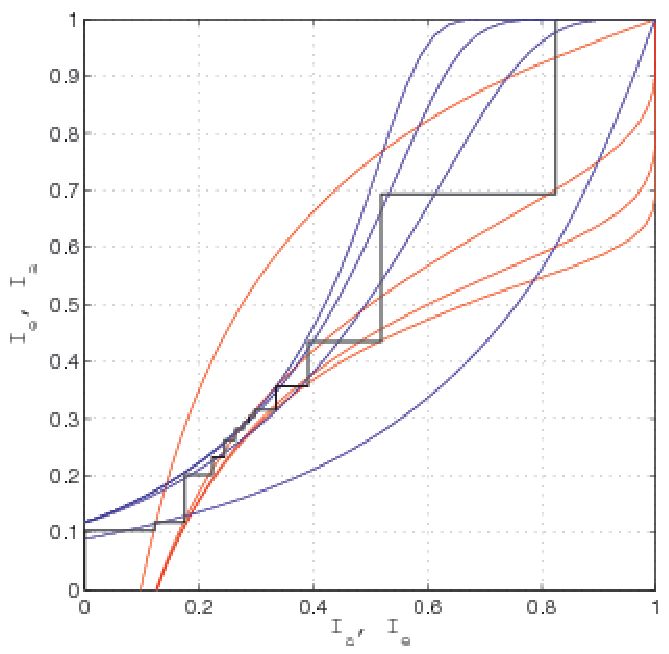
\includegraphics[width=7cm]{henkel_1}
 \caption{Convergence scheduling for hybrid concatenation}
%  \caption{Convergence scheduling for hybrid concatenation}
  \label{fig:henkel_1}
\end{figure}

In analog coding, we further improved the presentation of our proof that
Turbo-like decoding leads to a least-squares solution. We can now exactly
forecast the convergence limits for the stepsize and can also
modify it for every iteration to allow for very fast
convergence. For impulse-noise detection, we currently investigate new
statistical properties, e.g., the slope distribution, and correlation
approaches. This study will also close a gap in impulse-noise modeling
regarding the autocorrelation function of impulse noise.

By designing a new bit-allocation algorithm (pat. pending), following the
principles of an existing one by Chow, Cioffi, and Bingham, we can obtain UEP
properties in a very elegant way. It allows for an arbitrary number of
error-protection classes with arbitrary margins between them and an arbitrary
number of bits per class. Figure~\ref{fig:henkel_2} shows a resulting bit and
power allocation according to the channel SNRs, assuming three error protection
classes with a 3 dB separation.


\begin{figure}[ht]
  \centering
  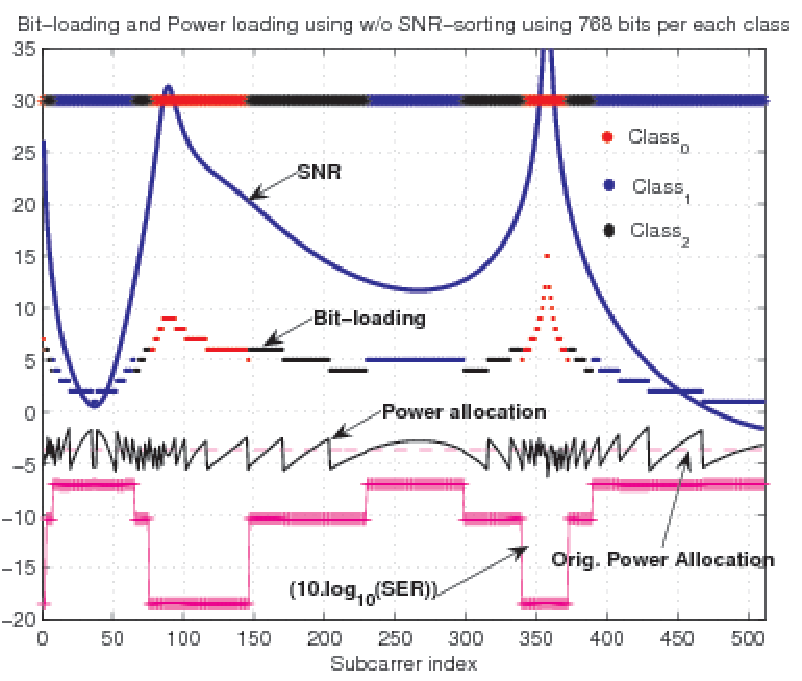
\includegraphics[width=7cm]{henkel_2}
  \caption{UEP bit and power allocation for three protection classes}
%  \caption{UEP bit and power allocation for three protection classes}
  \label{fig:henkel_2}
\end{figure}

\newpage
\paragraph{Organization}
% list the (research) events you have organized, if any,

\begin{enumerate}
\item Program Committee member of ICC 2006
\end{enumerate}

%\paragraph{Collaborations}
%\begin{enumerate}
%\item ...
%\item ...
%\item ...
%\end{enumerate}

\paragraph{Grants}
% list the running grants in 2005, if none have been received, please delete this
% subsection.
\begin{enumerate}
\item Funded by EU-IST STREP (FP 6), \emph{M-Pipe}, (October 2004
- March 2007)
\end{enumerate}

\paragraph{Patents}
\begin{enumerate}
\item  L. Sassatelli, W. Henkel, and D. Declercq. Check-Irregular LDPC Codes, Jan. 27
  2006. European Patent Application 06 100 979.1.
\item W. Henkel and K. Hassan. Unequal Error Protection Bit Loading for Multi-Carrier
  Transmission, Aug 30 2006. European Patent Application 06 119 771.1.
\end{enumerate}


%\paragraph{Publications}
% list the publications of 2005 (also accepted and in press), if none have been received, plese delete this
% subsection. Enter the publications into the SES publications database at
% http://kwarc.eecs.iu-bremen.de/ses-pubs/index.php and only reference them here.

%\begin{description}

%\item[Conference Proceedings]
  \nocite{Henkel_vDeetzen_IZS}
  \nocite{Hu_Henkel_Turbo}
  \nocite{Sassatelli_Henkel_Declercq_Turbo}
  \nocite{vDeetzen_Henkel_ISIT}
  \nocite{Henkel_Hassan_OFDM}
  \nocite{vDeetzen_ITG}
  \nocite{Hassan_Henkel_ITG}
%\item[Patents]
%  \nocite{Sassatelli_Henkel_Declercq_EP}
%  \nocite{Henkel_Hassan_EP}
%\end{description}

%%% Local Variables:
%%% mode: latex
%%% TeX-master: "report"
%%% End:


\subsubsection{Networks and
Distributed Systems}\label{ict:cns:schoenwaelder} \index{Sch\"onw\"alder,
J\"urgen}

\paragraph{Research Team}
J\"urgen Sch\"onw\"alder (Professor), Ha Manh Tran (PhD Student), Vlad Balan (MSc
Student), Mat\'u\v{s} Harvan (MSc Student), Vladislav Marinov (MSc Student)\\

Computer networks such as the Internet continue to change many aspects
of our daily life. The networks and protocols research group carries
out research related to Internet protocols, with strong relationships
to work undertaken by the Internet Engineering Task Force (IETF), an
organization responsible for Internet protocol standardization, and
the Internet Research Task Force (IRTF), an organization responsible
for longer-term research related to Internet protocols.

\paragraph{Highlights}

The operation of increasingly complex communication networks requires
supporting systems, so called network management systems.  Network
management protocols and associated data definitions have been
developed and standardized over the last decade to support open,
vendor-neutral access to management and control information.  While
some of these technologies are in wide-spread usage, there is little
information how the underlying protocols are utilized and what the
specific characteristics of network management interactions are. As a
consequence, there are no well accepted models which can be used to
analyze the impact of protocol changes.

\begin{figure}[ht]
  \begin{center}
     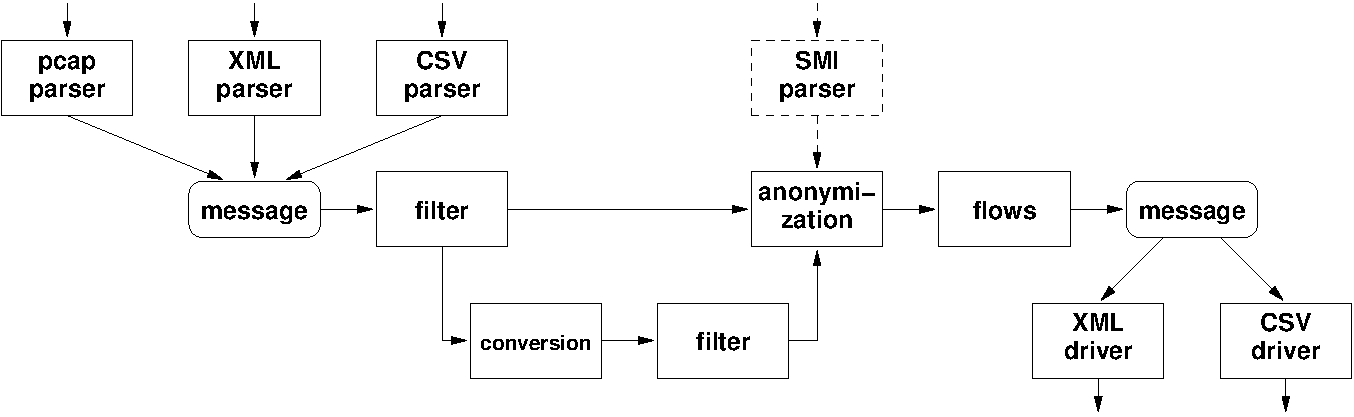
\includegraphics[width=\hsize]{schoenwaelder-tools}
  \end{center}
  \caption{Data flow within the \texttt{snmpdump} tool}\label{fig:snmpdump}
\end{figure}

A larger empirical study has been started in 2006 where we collect network management
packet traces from operational networks. This study is carried out in collaboration with
international research groups and supporting operators in order to obtain traces from live
networks. Based on an anonymization algorithm developed in 2005 \cite{HS06}, our group has
designed and implemented a tool chain (Fig.~\ref{fig:snmpdump}) for the analysis of
network management traffic traces \cite{PSHSM07}. Further research is ongoing to develop
analysis algorithms able to infer high-level management operations from observed primitive
protocol operations.

\begin{figure}[ht]
  \begin{center}
     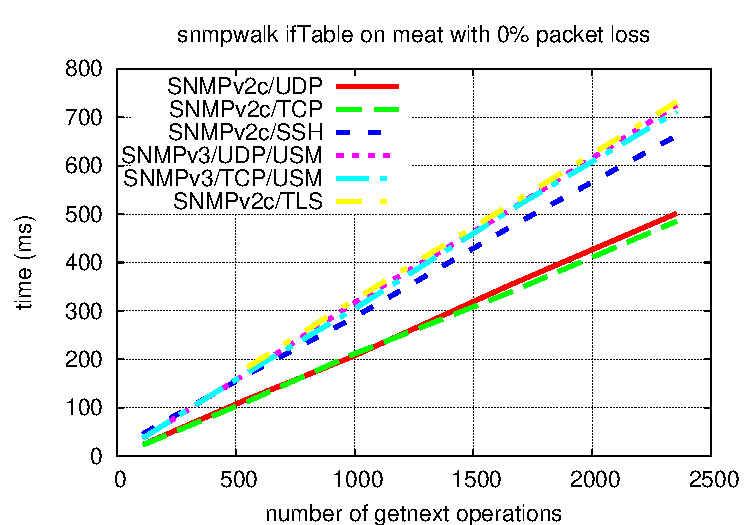
\includegraphics[width=\hsize]{schoenwaelder-sec}
  \end{center}
  \caption{Latency of SNMP/SSH and SNMP/TLS}\label{fig:sshtls}
\end{figure}

A related activity concerns the security of network management
interactions (Fig.~\ref{fig:sshtls}). We have prototyped and analyzed
a security extension proposed for the SNMP which leverages transport
layer security protocols such as SSH or TLS \cite{MS06}. This work is
related to standardization efforts undertaken by the Integrated
Security Model for SNMP (ISMS) working group of the IETF.

\begin{figure}[ht]
  \begin{center}
     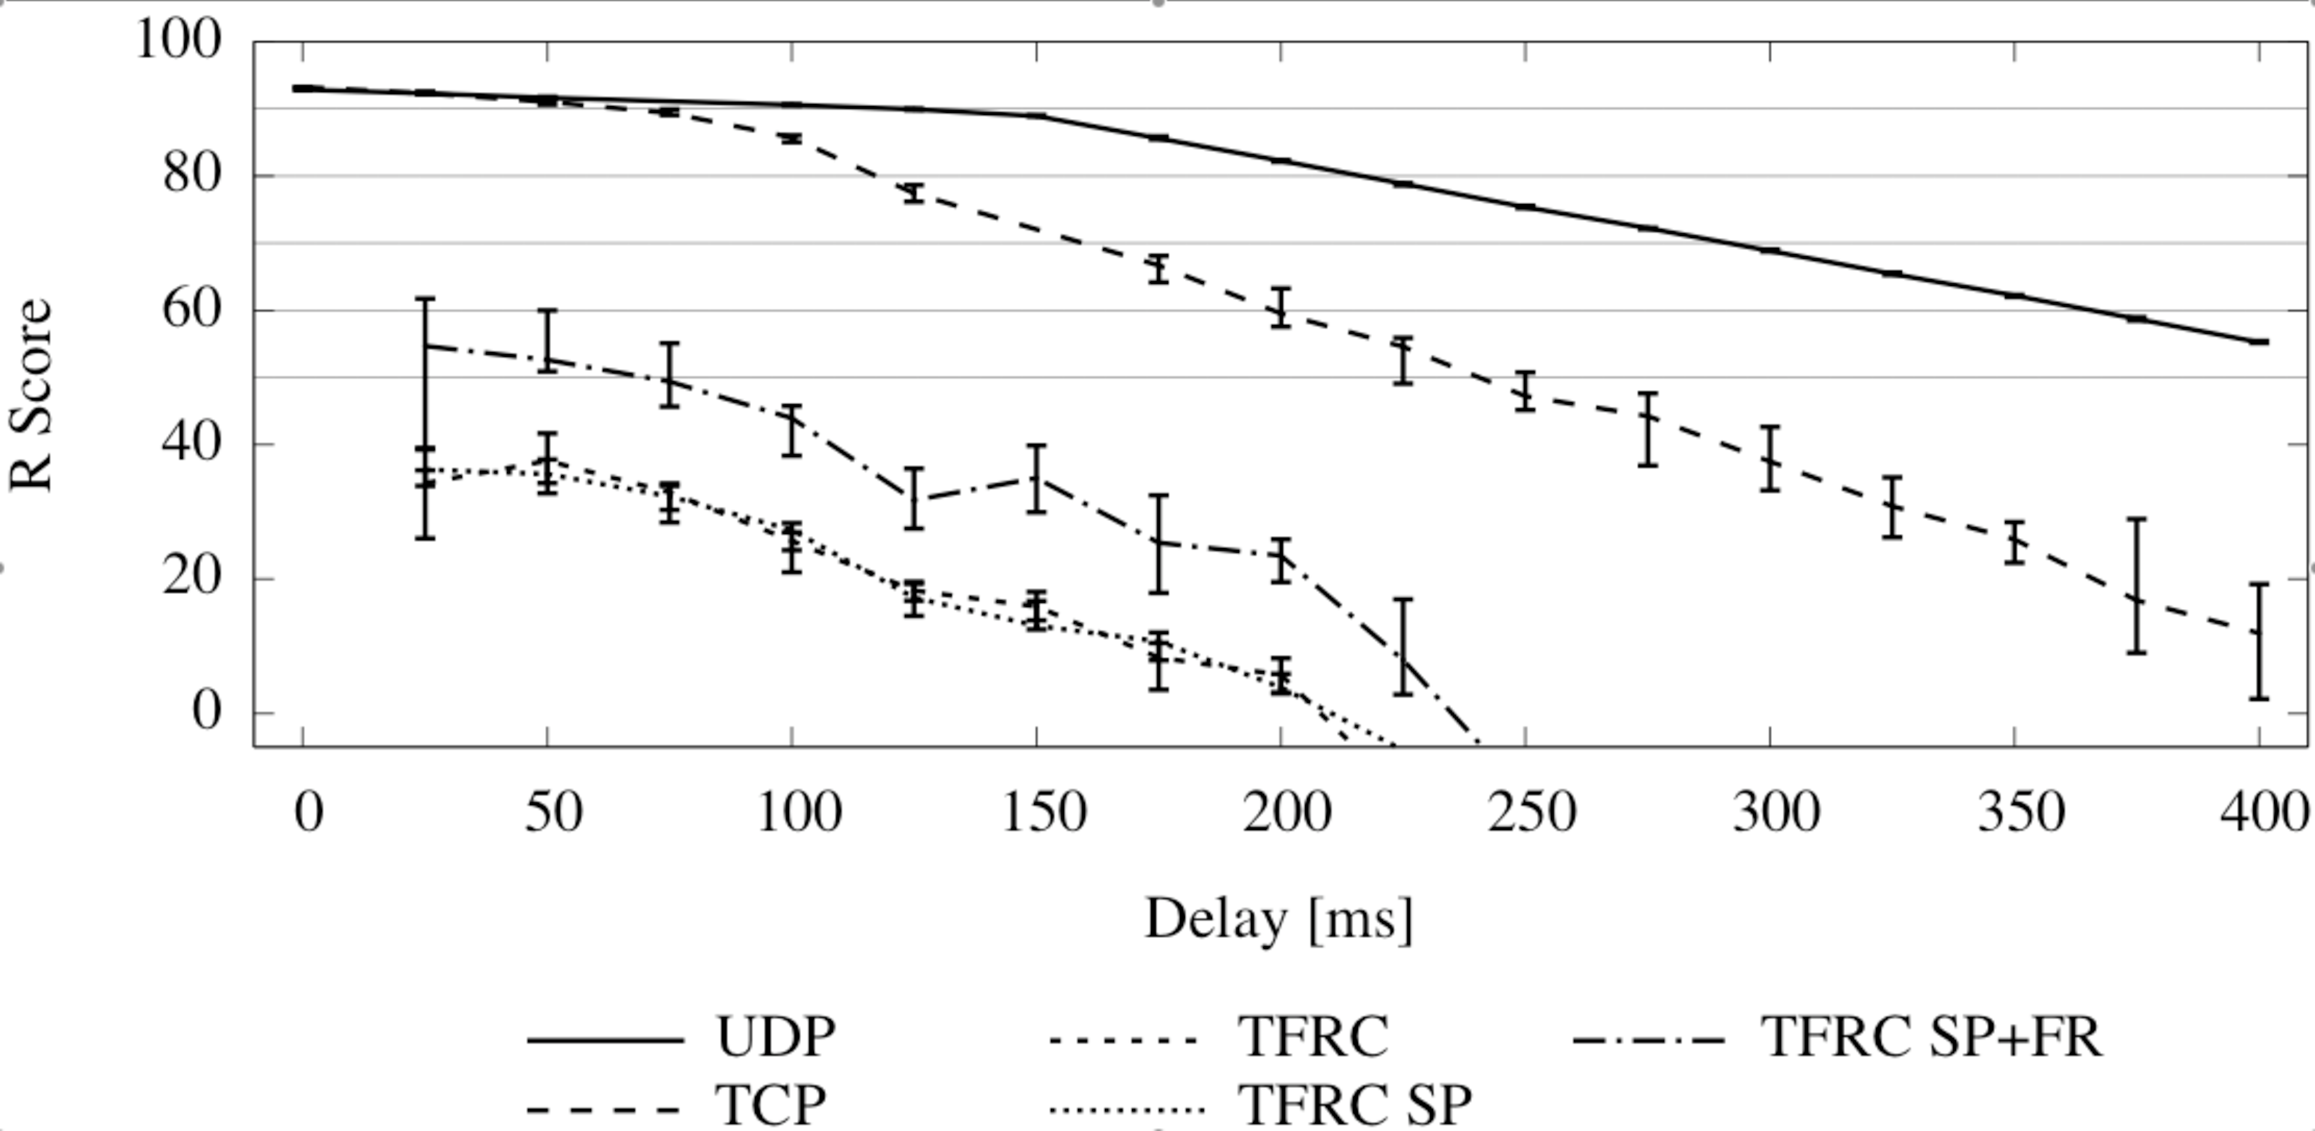
\includegraphics[width=\hsize]{schoenwaelder-dccp}
  \end{center}
  \caption{R scores for G.711 over DCCP}\label{fig:sshtls2}
\end{figure}

Finally, we have conducted research on the performance of voice stream
transmission over the new Data Congestion Control Protocol (DCCP)
being standardized by the IETF \cite{BENB07}. This work was carried out in
close collaboration with NEC C\&C Research in Heidelberg, Germany.


\penalty -50
\paragraph{Organization}\nobreak
% list the (research) events you have organized, if any,
\begin{enumerate}
    \item Editorial board member of the IEEE electronic Transactions on
          Network and Service Management
    \item Guest Co-Editor of a special issue on Peer-to-Peer
          Technologies in Network and Service Management of the
          Journal of Network and Systems Management
    \item Program Committee member of NOMS 2006, ACC 2006, DSOM 2006,
          IM 2007, ICCC 2007 NSO, SASO 2007, AIMS 2007
    \item Reviewer IEEE Communications Magazine, IEEE Transactions on
          Software Engineering, Springer Journal of Network and
      Systems Management
    \item Co-Chair of the IETF ISMS working group
    \item Member of the Security Directorate of the IETF
    \item Chair of the Network Management Research Group (NMRG) of the IRTF
    \item Chair of the 19th NMRG workshop on ``Promise Theory and New
          Approaches to Distributed Management'', KTH, Stockholm, January
          2006
    \item Chair of the 21st IRTF NMRG workshop on ``Future Direction
          of Network and Service Management Research'', SurfNet,
          Utrecht, October 2006
    \item Dissemination Activity Leader / Member of the Executive
          Committee of the EMANICS Network of Excellence
\end{enumerate}

\paragraph{Collaborations}
\begin{enumerate}
    \item {\sl University of Twente, The Netherlands}\\
          Prof.\ Aiko Pras\\
          Network Management, Traffic Measurements
    \item {\sl INRIA Lorraine, France}\\
          Prof.\ Olivier Festor\\
          Scalability of Management Protocols
    \item {\sl NEC C\&C Research}\\
          Dr.\ Lars Eggert\\
          Analysis of Voice over the Datagram Congestion Control Protocol
    \item {\sl NEC C\&C Research}\\
          Dr.\ J\"urgen Quittek\\
          Integrated Security Model for the Simple Network Management Protocol (SNMP)
    \item {\sl Huawei}\\
          David Harrington\\
          Architectural Models for Internet Management Protocols
    \item {\sl IEEE Project 802}\\
          Tony Jeffree\\
          SNMP over IEEE 802 Networks
\end{enumerate}

\paragraph{Grants}
\begin{enumerate}
    \item Funded by EU-IST NoE,  \emph{ ``EMANICS (EU Network of Excellence for the Management
      of Internet Technologies and Complex Services)''}, (January 2006 - December
      2009)
\end{enumerate}

%\paragraph{Awards, Prices}
%\begin{enumerate}
%\item IM 2005 Distinguished Experts Panel (invited panelist)
%\end{enumerate}

%\paragraph{Publications}

%\begin{description}
%  \item[Conference Proceedings]
  \nocite{HS06} \nocite{MS06} \nocite{BENB07}
  \nocite{PSHSM07} \nocite{DKPM07}
  %\item[Books/Collections]
  \nocite{Sch07}
 % \item[Standards]
  \nocite{RFC4789}
%\end{description}
%\end{document}
%%% Local Variables:
%%% mode: latex
%%% TeX-master: "report"
%%% End:

\subsubsection{Machine Learning}
\index{Jaeger, Herbert}
\paragraph{Research Team}
Herbert Jaeger (Professor), Mingjie Zhao (Postdoctoral Fellow), Mantas Lukosevicius (PhD student)\\


Herbert Jaeger and his team develops Machine Learning methods for
the automated construction of prediction models from empirical
time series data.  Target applications (and collaborations) are in
the fields of neurobiology, human music understanding, handwriting
recognition, control engineering and telecommunication. Two main
methods investigated in Herbert Jaeger's group are recurrent
neural networks of the ``Echo State Network'' (ESN) type and
observable operator models (OOMs). ESNs are interesting not only
because they yield highly efficient learning algorithms but also
because they offer a biologically plausible model of learning in
natural brains. OOMs generalize hidden Markov models, a standard
tool in speech and text recognition, yielding more expressive
models in a fraction of the learning time required for hidden
Markov models. Both ESNs and OOMs have been originally found by
Herbert Jaeger and have been investigated in his group over the
last few years.



\paragraph{Highlights}

An important application of machine learning methods for time series
data is speech recognition. Almost all current methods in this field
rely on ``hidden Markov models'' as the basic machine learning
technique. Although recurrent neural networks (RNNs) would be more
plausible from a bionics perspective -- after all, our brains are RNNs
--, and although it is known that artificial RNNs can, in principle,
yield optimal speech signal decoders, these models have not in
practice been used due to the extreme computational cost and the
danger of instability of previously known training methods for RNNs.
RNNs of the Echo State Network type are computationally cheap to train
and intrinsically stable. Thus, one research direction in Jaeger's
group is to tailor ESNs to speech processing tasks.

A widely used benchmark task in this field is the ``Japanese Vowels''
problem\footnote{Data donated by Mineichi Kudo, Jun Toyama, and Masaru
  Shimbo; obtainable at \url{http://kdd.ics.uci.edu}}. The training
data consist of pre-processed vocal recordings from 9 Japanese
speakers, with 30 recordings per speaker. The task is to train from
these data a classificator that can recognize the speaker in test
recordings. Figure \ref{fig:JaegerFig1} shows some recordings from the
training set. The task is difficult because of high intra-speaker
 and low inter-speaker  variability. The best known classification
 methods achieve a test error rate of slightly less than 2 \%. Using
 ESN-based models with an unconventional architecture (combining the
 classification ``votes'' of 1,000 tiny ESNs with a particular neuron
 model which is more biologically plausible than standard artificial
 neuron models), Jaeger et al.\ achieved a \emph{zero} test error
 \cite{Jaegeretal2}.

\begin{figure}[ht]
  \begin{center}
   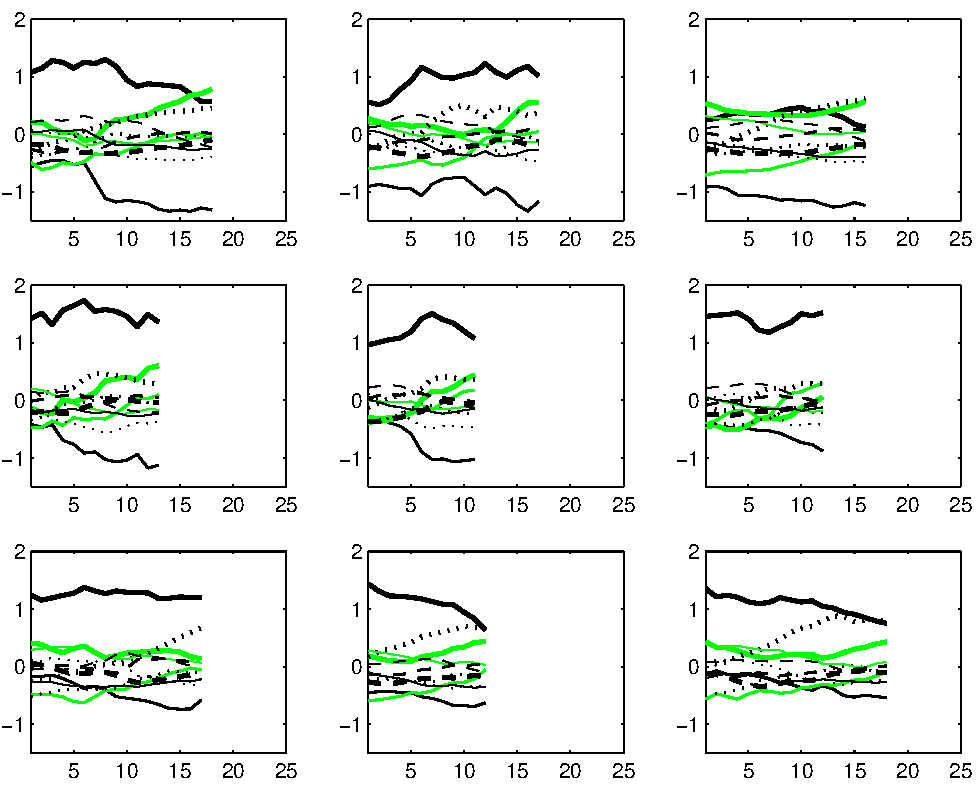
\includegraphics[width=\hsize]{JaegerFig1_2006.pdf}
    \caption{Some samples from the ``Japanese Vowels'' benchmark dataset. Each
    row shows three recordings from one speaker.}\label{fig:JaegerFig1}
   \end{center}
\end{figure}

Another important application of machine learning methods for time
series data is the recognition of handwritten texts. This task occurs,
for instance, in automated check reading systems or automated mail or
parcel sorting facilities. The text that is to be recognized is read
from left to right with a video reading head, yielding a video
sequence much like the visual input used by humans who read a text.
One difficulty in this domain arises from the circumstance that
handwritings can be narrow or stretched -- and this may even change
within a single written text. This is known as ``time warping''. An
automated reading system must be able to accomodate itself online to
changing character widths -- it must ``read faster'' when the
characters are narrow and ``read slower'' when they are
stretched. This poses a nasty chicken-and-egg problem: accomodation
would be easy if the characters were already recognized, but in order
to recognize them, the reading system must first accomodate to the
local ``writing speed''. Today's standard approach is to use dynamic
programming methods to optimize the local ``reading speed''. These
methods are computationally expensive and again, not biologically
plausible.

In a collaboration with Planet AG (Schwerin), a company specializing
in text recognition systems, a new ESN design was developed which
achieves an online accomodation to ``writing speed'' with no
additional computational cost, neither in the training phase nor in
the exploitation phase. So far, this
method was tested on synthetic data only, where it achieved a
close-to-optimal recognition performance \cite{Jaegeretal1,
  Jaegeretal2}. The collaboration with Planet AG will continue through
2007 and beyond.



\paragraph{Organization}
% list the (research) events you have organized, if any,

\begin{enumerate}
\item Interdisciplinary College 2006, G\"unne, Germany (member of program committee)
\item Studienstiftung Summer Academy Alpach 2006, Course ``Neuronal Plasticity'' (with D.\
  Jaeger, Emory University)
\item Special issue of \emph{Neural Networks} on ESNs and ``Liquid State Machines'', guest
  co-editor
\item ESN and ``Liquid State Machine'' workshop at NIPS 2006 (co-organizer)
\item Coordinator of a joint IUB -- University Bremen \emph{Exzellenzinitiative} proposal
  ``Bremen Graduate School for Computational Modeling of Complex Systems''
\end{enumerate}

\paragraph{Collaborations}
\begin{enumerate}
\item {\sl TU Graz} \\ Prof. Wolfgang Maass \\ Echo State Networks and Liquid State
  Machines
\item {\sl Planet AG, Schwerin} \\ Echo State Networks for handwriting recognition
\item {\sl Emory University, Atlanta} \\ Prof. Dieter Jaeger \\
  Biological and artificial models of neuronal plasticity
\item {\sl Universit\'e de Montr\'al} \\ Prof. Douglas Eck \\ Echo State Networks for
  music processing
\item {\sl Fraunhofer Institute IAIS, Sankt Augustin} \\ Prof. Paul
  Pl\"oger \\ ESNs for robot control
\item {\sl Universit�t K\"oln}\\ Dr. Alexander Sch\"onhuth \\ Mathematical theory of
  observable operator models
\end{enumerate}


\paragraph{Grants}
% list the running grants in 2005, if none have been received, please delete this
% subsection.
\begin{enumerate}
\item Funded by DFG, \emph {Quadratic observable operator models},
(December 2005 - December 2007)

\item Funded by private partner Planet AG, Schwerin,
\emph{Time-warping invariant echo
  state networks}, (September 2005 - August 2006)
\end{enumerate}

\nocite{Jaeger3}

%%% Local Variables:
%%% mode: latex
%%% TeX-master: "report"
%%% End:

\subsubsection{Harmonic Analysis applied to Communications
               Engineering}\label{ict:pfander}
               \index{Pfander, G\"otz}

\paragraph{Research Team}
G\"{o}tz Pfander (Professor), Niklas Grip (Postdoctoral Fellow)\\

%%% give a very short (150 words description of your research area)

In Multi-Carrier Modulation (MCM) communication schemes, the
channel input signal is synthesized as a linear combination
(superposition) of certain basis functions whose coeffcients
(weights) are bearing digital information. The performance of an
MCM system depends largely on the choice of the basis functions
which should allow the receiver to perform a fast and reliable
recovery of the transmitted information from the channel output.

For years, Orthogonal Frequency Division Multiplexing (OFDM) has
dominated MCM transmission systems, originally in time invariant
environments as in DSL applications but more recently also in slowly
time varying channels. The reason for this lies in the fact that, in
the stationary set-up, the OFDM carrier signals are approximate
eigenfunctions of the channel operator.

Mathematically, or more precisely, within harmonic analysis, OFDM
has been extensively studied under the disguise of Gabor analysis,
where stability issues, synthesis and analysis algorithms, and
carrier functions design are discussed at length (see also
Section~\ref{mps:pfander}).


\paragraph{Highlights}

In recent years, we have applied Gabor analysis to provide
mathematical contributions to MCM communications. For example, we
have shown that Gabor systems (OFDM, DMT) clearly outperform wavelet
systems (DWMT) in time invariant channels and we have analyzed
estimates of the crest factor of trigonometric polynomials which
underly OFDM.

In mobile and therefore wireless and time variant communication
environments, the transmitted signal reaches the receiver along a
continuum of different signal paths, each featuring a path dependent
time delay and a frequency shift caused by the doppler effect.
Nevertheless, physical constraints imply that this time--frequency
dispersion of the transmission signal is of limited extent. Hence,
wireless channels can be modelled by operators, which are weighted
superpositions of time and frequency shifts occupying a limited
region, the so--called spreading support in the time--frequency
plane. The weight functions are the so--called spreading functions
which play a fundamental role in our research
(Section~\ref{mps:pfander}).

\null {\emph{Transmission Basis Design:}} Since Fall 2004, we are
working on a DFG funded project, whose aim is the mathematical
analysis and optimisation of coded orthogonal frequency division
multiplexing (COFDM) in view of transmission stability in wireless
and other time variant environments. One of the cornerstones of
this project is the analysis of the perturbation stability of
different bases when used in wireless channels.

 \begin{figure}[ht]
   \begin{center}
    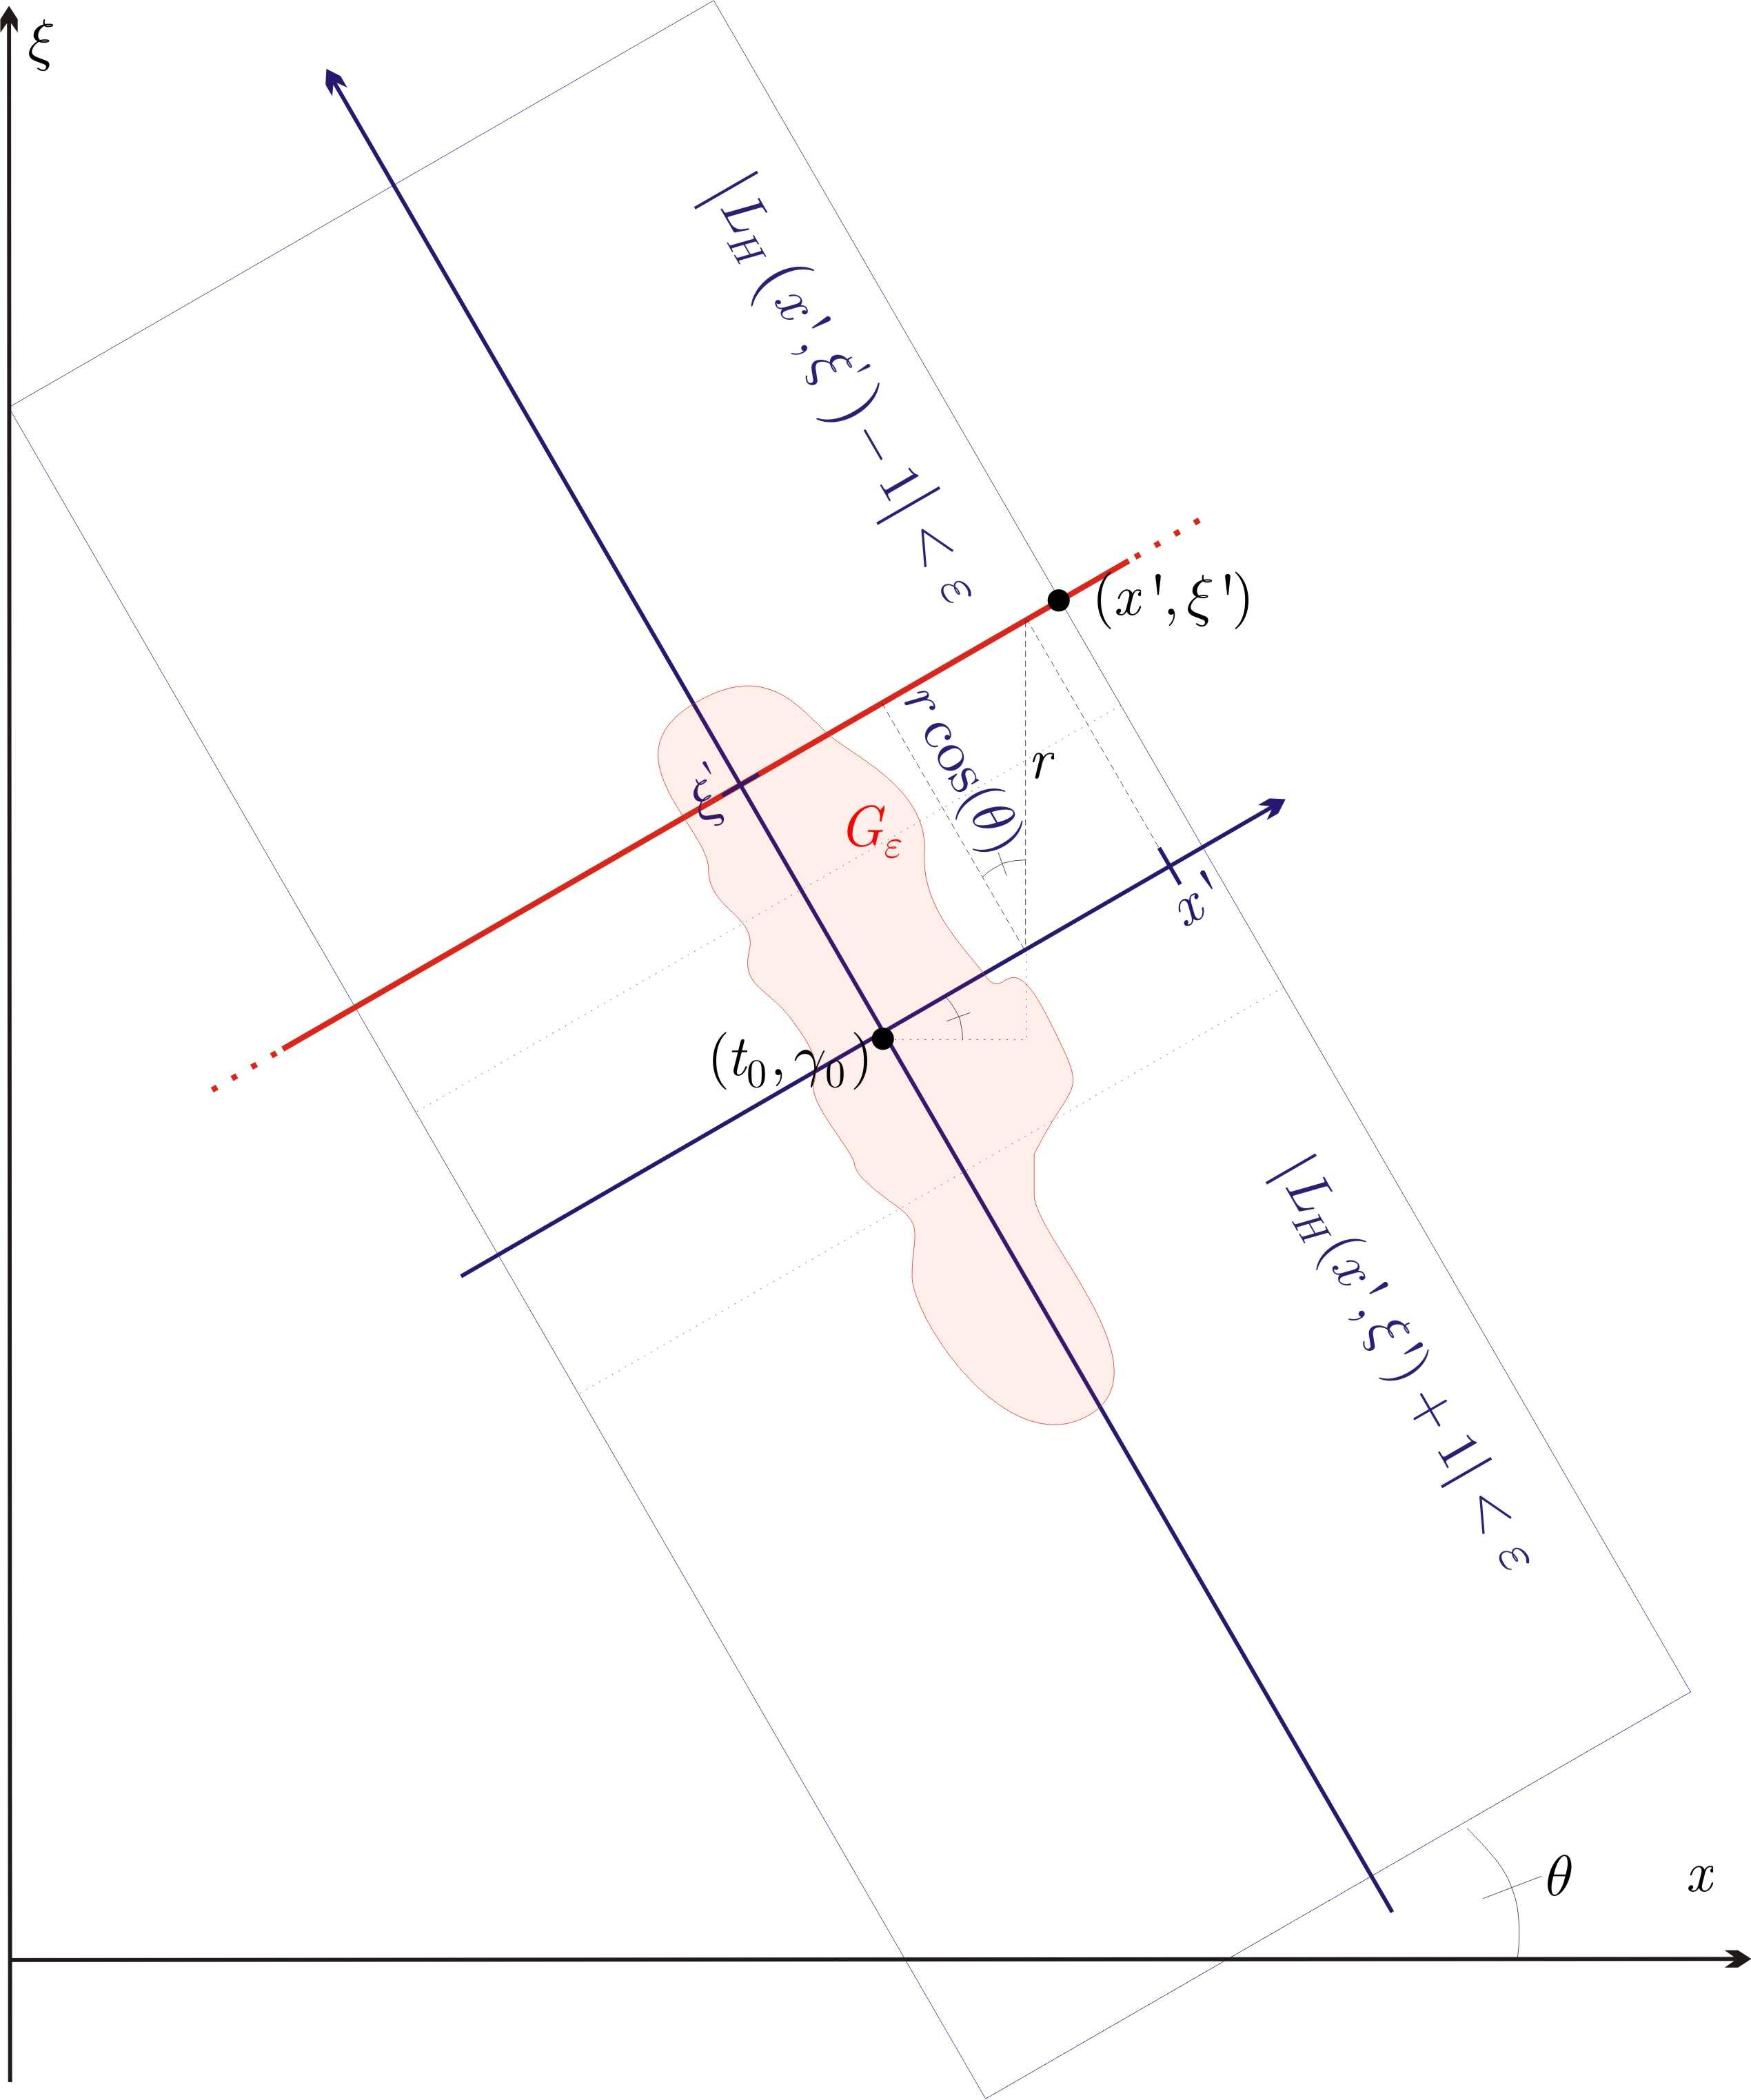
\includegraphics[width=7cm]{pfander.png}
     \caption{Construction of a channel spreading function whose operator causes a large distortion to a function
     with time--frequency $\epsilon$-support $G_\epsilon$.}
     \label{fig:pfander}
   \end{center}
 \end{figure}
% to reference it use ``Figure.~\ref{fig:xxx}''; the numbers will be computed automatically.

Within this realm, we derived estimates which relate the worst case
distortion of a function to the functions time--frequency
concentration and the channel operators spreading support (see
Figure~\ref{fig:pfander}). These results should, similarly to our
previous work on time invariant channels, allow us to show that OFDM
outperforms wavelet methods in mobile communication channels.

Further,  we continued our work on the modelling of narrowband
finite lifelength systems such as wireless radio communications by
smooth and compactly supported spreading functions. Our results were
used to derive a fast algorithm for computing the matrix
representation of a channel operator with respect to pulseshaped
OFDM bases \cite{GP06}.

\null {\emph{Operator/Channel Identification:}}  One of the key
problems in the design of elementary building blocks for mobile
communications is the incomplete knowledge of the ever--changing
transmission channels. The goal of operator/channel identification
is to obtain complete knowledge of a (channel-) operator by
observing the output caused by a single input signal.

Within the last years, we showed that classes of operators characterized by a bounded
spreading support region allow identification of its members if and only if the area of
the spreading support region is less than or equal to one, a phenomenon which is closely
related to Heisenberg's uncertainty principle~\cite{PW06,PW06b}. The theory, motivated by
communications engineering, has lead to the development of a sampling theory of operators
which is described in Section~\ref{mps:pfander}.

\null {\emph{Coding:}} Discrete, overcomplete Gabor systems can be
used to encode finite dimensional vectors in order to gain
robustness to errors introduced in  communications channels. In
\cite{KPR06}, we construct a large class of Gabor like equal norm
tight frames that are maximally robust to erasures. Further, we
discuss consequences of our findings to the theory of recovering and
storing signals which have sparse time--frequency representations.

%These results are further discussed in~\cite{KPR05}. The main
%focus of this paper are uncertainty principles for time--frequency
%representations of vectors in  finite dimensional vector spaces
%(Section~\ref{mps:pfander}).

%Possibly Channel matrix as picture
%
%% to include a figure, generate a file xxx.pdf and integrate the following lines
%\begin{figure}[ht]
%  \begin{center}
%   \includegraphics[width=10cm]{Pfander.pdf}
%    \caption{The caption of the figure}
%    \label{fig:xxx}
%  \end{center}
%\end{figure}
%% to reference it use ``Figure.~\ref{fig:xxx}''; the numbers will be computed automatically.
%
% Text ....
%
%
%\paragraph{Organization}
%% list the (research) events you have organized, if any,
%
%\begin{enumerate}
%\item  ....
%\item   ...
%\item  ...
%\end{enumerate}

\null G\"otz Pfander is also involved in  ``Applied Mathematics''
(Section~\ref{mps:pfander}).

\paragraph{Collaborations}
\begin{enumerate}
    \item {\sl International University Bremen}\\
          Prof. Harald Haas, Prof. Werner Henkel\\
          Design of OFDM systems for time--varying channels
    \item {\sl George Mason University, USA}\\
          Prof. David Walnut\\
          Operator sampling and channel measurements
    \item {\sl Numerical Harmonic Analysis Group and European Center
          for Time--Frequency Analysis, Vienna University, Austria}\\
          Prof. Hans Feichtinger, Prof. Karlheinz Gr\"ochenig\\
          Gabor analysis and applications to mobile communications
\end{enumerate}

\newpage
\paragraph{Grants}

\begin{enumerate}
    \item Funded by DFG, \emph {Analysis and design of COFDM multicarrier modulation techniques in view
          of transmission stability in time variant channels}, (September 2004 - December
          2006)
\end{enumerate}

%
%\paragraph{Patents}
%% list the grants you have received in 2005, if none have been received, plese delete this
%% subsection.
%\begin{enumerate}
%\item
%\item
%\end{enumerate}
%

%\paragraph{Awards, Prices}
%% list the grants you have received in 2005, if none have been received, plese delete this
%% subsection.
%\begin{enumerate}
%\item
%\item
%\end{enumerate}

%\paragraph{Publications}
% list the publications of 2005 (also accepted and in press), if none have been received, plese delete this
% subsection. Enter the publications into the SES publications database at
% http://kwarc.eecs.iu-bremen.de/ses-pubs/index.php and only reference them here.

%\begin{description}
 % \item[Journals]  Journal of Fourier Analysis and
 % Applications~
  %\nocite{LPW05,Pfa05}
 % \item[Submitted] IEEE Transactions on Information
%  Theory~
  %\nocite{PW051,GP05}
%\item[In preparation]
%\nocite{Pfa05b,KPR05}
%\end{description}


%\bibliographystyle{alpha}
%\bibliography{report-pfander-2005}

%\end{document}
%%% Local Variables:
%%% mode: latex
%%% TeX-master: "report"
%%% End:

\subsubsection{Channel Characterization, Electromagnetics, Prototype System Development}
\index{Wallace, Jon}

\paragraph{Research Team}
Wallace, Jon (Professor)\\

Research combines the diverse areas of electromagnetics and
propagation, signal processing, and communications, to allow more
accurate modeling of realistic communications systems, revealing how
to optimize the performance of complex systems as a whole rather
than just the constituent parts.  This research involves a strong
experimental component, allowing results to be based on real-world
experiments and measurements and not just theoretical analysis. This
effort has led to the development of a number of prototype
multiple-input multiple-output (MIMO) wireless channel sounders and
the fabrication of RF/microwave antennas and components,
facilitating the development of accurate channel models and
revealing the impact of factors such as antenna mutual coupling,
directivity, and polarity. The work also encompasses the development
of real-time systems based on DSP and FPGA architectures for
implementing proposed communications algorithms as well as advanced
measurements techniques.

\paragraph{Highlights}

The work during 2006 has focused primarily on understanding the
complex behavior of time-varying MIMO wireless channels.  The rate
of time variation determines whether the MIMO communications channel
can be adequately tracked, allowing high throughput to be achieved
with the multiple antennas.

\begin{figure}[ht]
  \begin{center}
    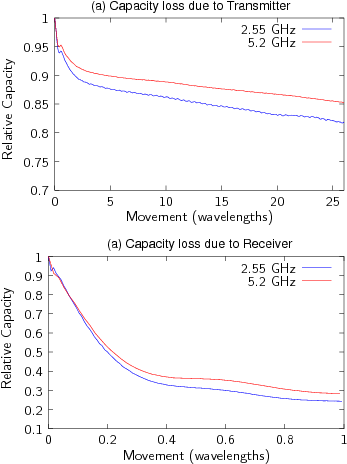
\includegraphics[width=6cm]{wallace_cap_deg.png}
    \caption{Capacity loss from time-varying channel with receiver
    movement due to channel errors at (a) transmitter and (b) receiver}
   \label{fig:wallace_cap_deg}
   \end{center}
\end{figure}

Measurement and analysis of time-varying channels in indoor and
outdoor environments at different frequencies revealed that for
moving users, the channel must be sampled at the receiver
approximately every 0.1 wavelength or shorter for high-capacity
communications, as depicted in Fig.~\ref{fig:wallace_cap_deg}.  It
was also found that channel information at the transmitter is less
critical and can be updated at the slower rate of every 1 wavelength
for high capacity.

This study on channel time-variation also led to metrics that quantify
the impact of the temporal variability as well as accurate methods of
capturing this behavior in computer simulations.  For very rapidly
fading channels (where learning the channel is not possible) it was
discovered that mutual coupling of the transmit array is a critical
factor affecting the system performance, and that not including
mutual coupling in the system model leads to erroneous conclusions
about the optimal configuration of the transmit antenna array.

\begin{figure}[ht]
  \begin{center}
    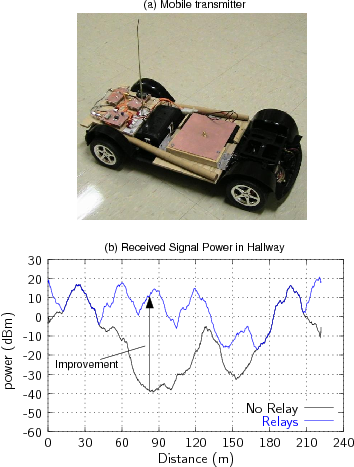
\includegraphics[width=6cm]{wallace_relay2.png}
    \caption{System for rapid shadowing/pathloss measurements and possible
    improvement using relays for a hallway environment}
   \label{fig:wallace_relays}
   \end{center}
\end{figure}

Additional channel modeling work done in collaboration with the
University of Pretoria, South Africa, has demonstrated interesting
properties of indoor propagation channels.  It has been discovered
that the multipath structure, antenna correlation, and channel
capacity are very similar, even when the center frequency is scaled.

Defense-related contract work  was done for San Diego Research
Corporation, USA, whose primary goal was to quantify how the
blockage (or shadowing) of electromagnetic signals in urban
environments limits communications reliability, and whether this
could be improved by robotic relays.  As depicted in
Fig.~\ref{fig:wallace_relays}, a transmitter operating at 300 MHz,
900 MHz, and 2 GHz, was mounted on a remote control car and the
signal strength was measured on a fixed receiver.  The car was
driven in many different scenarios: indoor hallway, indoor room,
outdoor-to-indoor channels, behind automobile, under automobile,
etc. Analysis of the resulting shadowing versus position revealed
that shadowing can cause a drop of 10-30 dB when going around a
corner or behind an automobile.  A simple daisy-chain relay model,
however, indicated that self-configuring robotic relays may be
effective in allowing reliable communications in these environments.


In the future, the main focus is  building up new experimental
capability for ultrawideband multiple antenna channel sounding and
cognitive radio, as well as forming collaborative relationships with
other key researchers in Germany and Europe.

%Pictures are to be included via:
%
%\begin{figure}[ht]
%  \begin{center}
%    \includegraphics[width=6cm]{profxxx-figx.jpg}
%    \mycaption{ xxx )}\label{fig:profxxx}
%   \end{center}
%\end{figure}

% \paragraph{Organization}
% list the (research) events you have organized, if any,
%
%\begin{enumerate}
%\item  xxx
%\item  xxx
%\end{enumerate}

 
\paragraph{Collaborations}
\begin{enumerate}
\item {\sl University of Pretoria, South Africa} \\ B. T. Maharaj and L. P. Linde \\ Indoor Channel Measurement and Modeling
%\item {\sl Institution} \\ Partner \\ Research Topic \ Collaboration
\end{enumerate}

%\paragraph{Grants}
%% list the running grants in 2005, if none have been received, please delete this
%% subsection.
%\begin{enumerate}
%\item {Funded by} ``Proposal ��
%\item {Funded by} ``Proposal ��
%\end{enumerate}

%\paragraph{Awards, Prizes}
%% list the grants you have received in 2005, if none have been received, please delete this
%% subsection.
%\begin{enumerate}
%\item
%\item
%\end{enumerate}

%\paragraph{Publications}
  \nocite{wallace_06bWALa,wallace_069WAL,wallace_06bWALb}

%Publications should be delivered as a separate file (naming
%convention profxxx.bib. See description by R. Helling. Please make
%sure that all your publications are referred to in the TiX file.
%This can either be in form of a \cite{profxxxkey} or as a
%\nocite{profxxxkey} in the end. A publication which is not
%reffered to on the LaTeX file doesn't produce any output in the
%report.


\shorttitle{Robotics and Embedded Systems}%
\subsection{Robotics and Embedded Systems} %
Robotics is the driving force behind the increasing omnipresence
of automation, not only in industry but also in many areas of our
daily lives. In addition to their well-established role as
programmable machine-tools, robots are more and more used in
domains where some autonomy and intelligence is necessary, where
the system is not constantly supervised by a human operator and
where it has to be adaptive as the developer of the system can not
fully predict which situations the system will encounter in its
application environment. The related computer hardware and
software are the key ingredients of robots.

%%% Local Variables:
%%% mode: latex
%%% TeX-master: "report"
%%% End:

\subsubsection{Robotics}\label{ict:robotics:birk}
\index{Birk, Andreas}

\paragraph{Research Team}
Andreas Birk (Professor),
Kaustubh Pathak (Postdoctoral Fellow),
Winai Chonnaparamutt (PhD Student),
Mohammed Nour Abdel-Gwad Ahmed (PhD Student),
Max Pfingsthorn (PhD Student),
Jann Poppinga (PhD Student),
S\"{o}ren Schwertfeger (PhD Student) \\

The research of the Birk group focuses on Autonomous Systems. The work ranges from the
development of embedded hardware via mechatronics and sensors to high-level software. On
the basic research side of autonomous systems, machine learning and cooperation are core
activities. The robotics systems developed are used in various domains including
underwater and especially rescue robots.

 Especially mobile robots can be highly valuable tools in urban rescue
missions after catastrophes like earthquakes, bomb- or gas-explosions or daily incidents
like fires and road accidents involving hazardous materials. The robots are used to
inspect collapsed structures, to assess the situation and to search and locate
victims. There are many engineering and scientific challenges. Rescue robots not only have
to be designed for the harsh environmental conditions of disasters, but they also need
advanced capabilities like intelligent behaviors to free them from constant supervision by
operators.  IUB robotics is among the world-wide leading groups in this domain.

\paragraph{Highlights}

The IUB rescue robots demonstrated their capabilities on several
occasions including technology demonstrations, especially the Rescue
Robot Field Test Demo (figure~\ref{fig:outdoor}) and the European
Land Robotics Trials (ELROB). The robots also demonstrated their
capabilities at several competitions, namely three RoboCup events.
At the RoboCup US Open in Atlanta, the IUB team won the first place
in the rescue robot league, beating the favored US American groups.
The team also won the first place at the European RoboCup
competition, the Dutch Open in Eindhoven. The team also got the
Innovation Award at the RoboCup World Championship in Bremen for
demonstrating for the first time the successful combined usage of a
tele-operated with a fully autonomous robot at rescue missions. IUB
was the only European team that made it to the final round at the
RoboCup World Championship, and it was beaten in the end by Asian
teams that purely relied on tele-operated devices without any
on-board intelligence.



\begin{figure}[thpb]
  \centering
  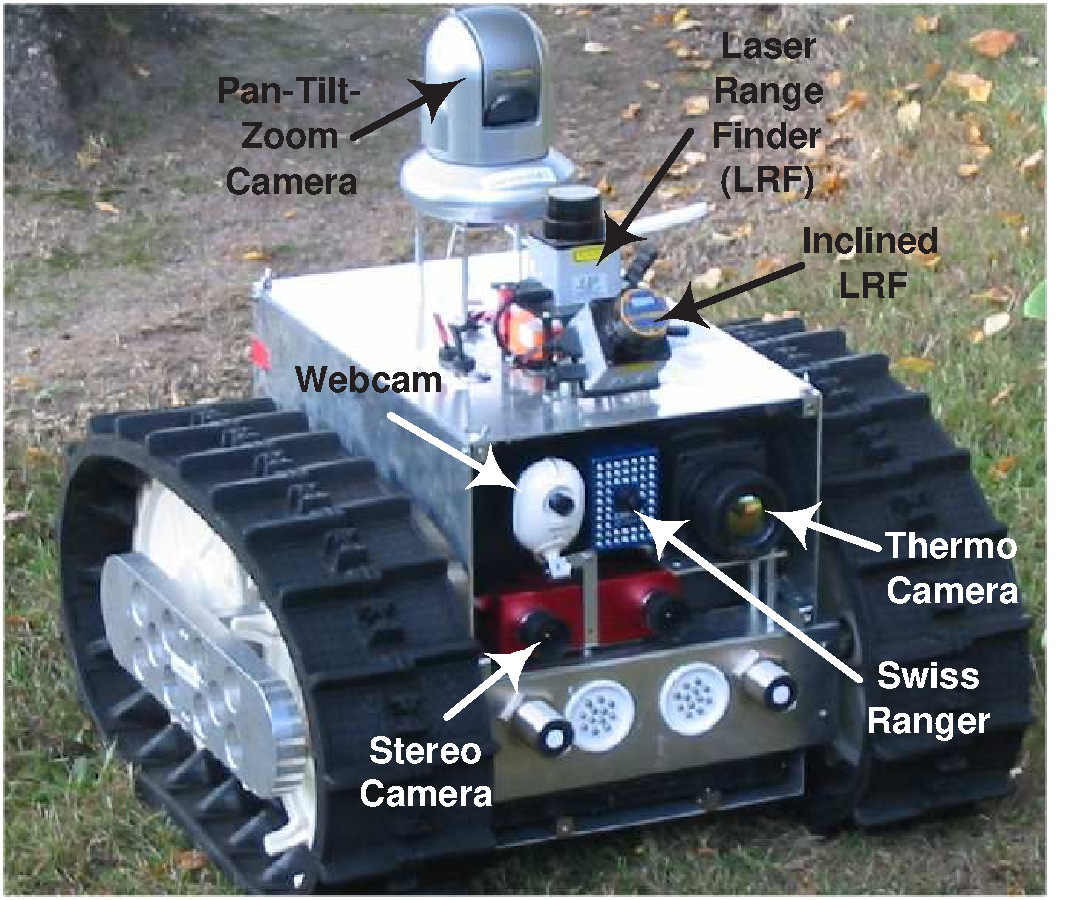
\includegraphics[width=\linewidth]{autonomousrobot.pdf}
  \caption{A {rugbot} with a selection of on-board sensors. Several sensors are dedicated
    to 3D range sensing to generate 3D environment models with a novel approach.}
  \label{fig:rugbot}
\end{figure}




On the research side, several contributions have been made ranging from the robot
mechatronics over on-board intelligence up to cooperative systems level.  Regarding the
mechatronics of the robots, a new locomotion system \cite{birk_flipper_rcup06} and a
special mobile communication system were developed \cite{birk_rescuecabledrum_rcup05}. The
latest type of robot from IUB robotics, the so-called rugbot, short for rugged robot, is
meanwhile one of the most advanced systems in this field \cite{birk_rugbot_ssrr06}. But
this holds not only for its mechatronic side but especially also with respect to its
on-board intelligence going up to full autonomy
\cite{birk_rescueteam_rcup05}. Contributions to several core topics for intelligent mobile
robot have been made in this context, especially for map generation
\cite{birkRescRobARJ06}, for the vectorization of maps
\cite{birk_mapvectorization_rcup06}, for the integration of autonomous behaviors with user
interactions \cite{birk_rescueGUI_rcup05}, and for the underlying architecture for
autonomy \cite{birk_autonomy_ssrr06}. The group also contributed to a high fidelity
simulator for mobile robots \cite{birk_virtualrobot_rcup05} that plays a significant role
in the prototype development of intelligent robot software.  Last but not least, work
regarding cooperative robot teams was done. The contributions include a novel algorithm
for multi robot exploration \cite{birk_CommExpore_CEP06} that can be used for search and
rescue missions by robot packs \cite{birk_commexplore_rcup05}. A second important result
is a novel algorithm for multi robot mapping \cite{BirkMultiMap_IEEEproc}.


\begin{figure*}
\centering
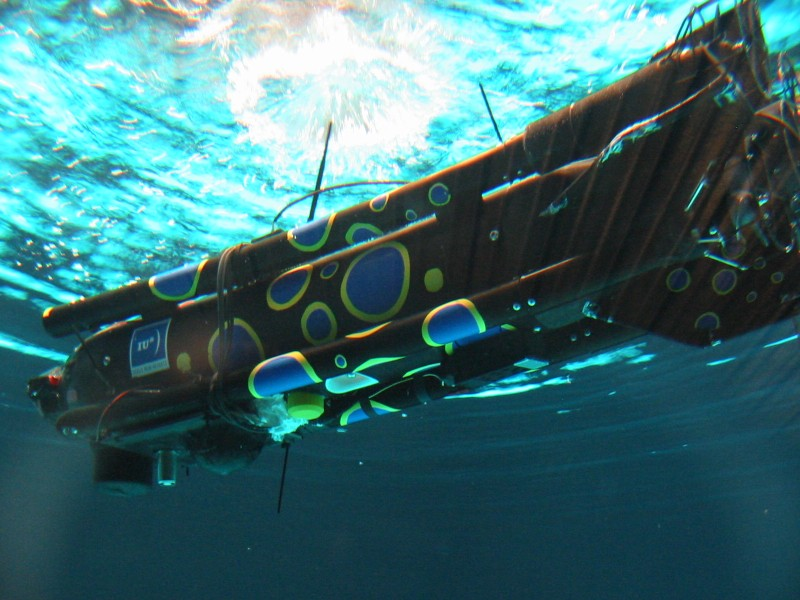
\includegraphics[width=.32\linewidth]{AUV-2006-best01.png}
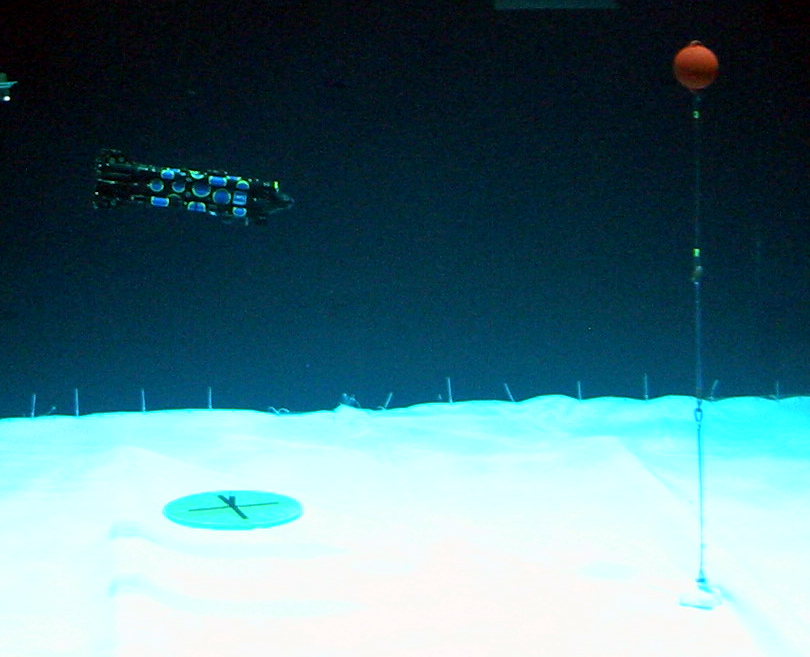
\includegraphics[width=.32\linewidth]{AUV-2006-best03.png}
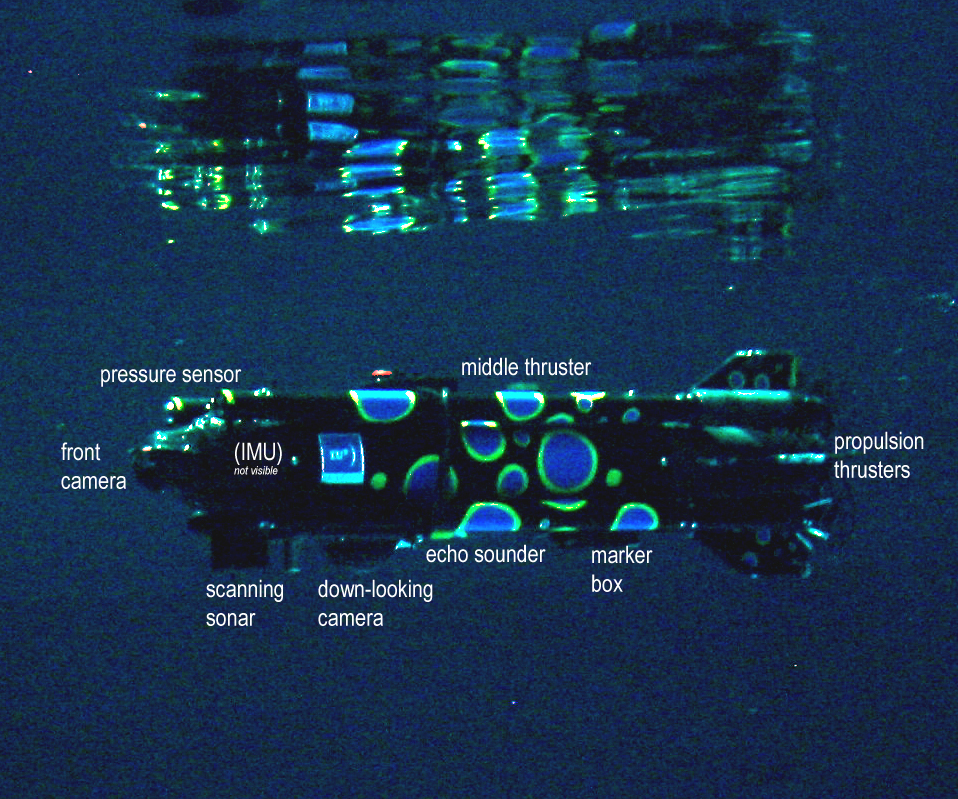
\includegraphics[width=.32\linewidth]{AUV-2006-best02-text.png}
\caption{The IUB-ATLAS Autonomous Underwater Vehicle (AUV) diving in a test pool
  (left). The AUV on an autonomous mission, searching for a midwater target in form of a
  submerged orange buoy (center). An overview of the main sensors of the AUV (right).}
\label{IUB-AUV}
\end{figure*}

IUB robotics made in 2006 also first successful practical steps in the domain of
underwater robotics by developing an Autonomous Underwater Vehicle (AUV). The work was
jointly done with ATLAS Elektronik in a cooperative project including also the IUB
robotics club. The most basic vehicle parts, namely the hull, the batteries, the motors
with propellers, and some sensors were provided to IUB by ATLAS. The on-board control
electronics and software were completely developed by IUB. This work is based on the
CubeSystem, a collection of hard- and software-components for fast robot prototyping,
which is also used for the IUB land robots. The AUV features fully autonomous motion
control and mission planning. It has an on-board vision system that allows to recognize
targets and to trigger appropriate behaviors. The system already successfully demonstrated
its capabilities at the Student Autonomous Underwater Challenge - Europe (SAUC-E), which
took place in August at the Pinewood movie studios near London.  The IUB-ATLAS-AUV came in
on second place in the performance evaluations, beating several of the established
underwater robotics research institutions.

\paragraph{Organization}
% list the (research) events you have organized, if any,

\begin{enumerate}
\item Chair ``RoboCup World Championship 2006, Rescue Robot League'', Bremen, Germany
\item Organizer ``Rescue Robot Field Test Demo'', opening event of RoboCup World
  Championship 2006, Bremen, Germany
\item Program Committee Member/Reviewer: Journal of Robotics and Autonomous Systems;
  Journal of Control Engineering Practice; International RoboCup Symposium; IEEE
  International Workshop on Safety, Security, and Rescue Robotics
\end{enumerate}

\paragraph{Collaborations}
\begin{enumerate}
\item {\sl International Rescue Systems Institute, Kobe, Japan}\\
  Prof. Satoshi Tadokoro\\
  Rescue Systems and Applications
\item {\sl University of Rome ``La Sapienza'', Italy}\\
  Prof. Daniele Nardi\\
  Autonomous Intelligent Functionalities within Rescue Robotics
\item {\sl Imperial College, London, UK}\\
  Dr. Yiannis Demiris, Senior Lecturer\\
  World Modeling by Autonomous Intelligent Systems
\end{enumerate}

\paragraph{Awards, Prizes}
\begin{enumerate}
\item Innovation Award, "Best Mixed Initiative Team"; RoboCup World Championship; Rescue
  Robot League; Bremen, Germany; July 2006
\item 1st Place Team; RoboCup US Open, Rescue Robot League; Atlanta, USA; April 2006
\item 1st Place Team; RoboCup Dutch Open, Rescue Robot League; Eindhoven, Netherlans; April 2006
\end{enumerate}

\paragraph{Grants}
% list the running grants in 2005, if none have been received, please delete this
% subsection.
\begin{enumerate}
\item Funded by DFG,  \emph{Learning of 3-Dimensional Maps of
Unstructured
Environments on a Mobile Robot}, May 2005 - April 2008 \\


\item Funded by DAAD-PPP,  \emph{3D Wordmodeling for Robot Action
Planning, Recognition and Imitation}, (July 2006 - June 2008) \\


\item Funded by private partner ATLAS Elektronik,
\emph{IUB-ATLAS Autonomous Underwater Vehicle}, (February 2006 - July 2006)\\


\item Funded by EU-IST NoE \emph{EUropean RObotics research
Network (EURON)}, (May 2004 - April 2008)

\end{enumerate}

%\paragraph{Publications}
% list the publications of 2005 (also accepted and in press), if none have been received, plese delete this
% subsection. Enter the publications into the SES publications database at
% http://kwarc.eecs.iu-bremen.de/ses-pubs/index.php and only reference them here.

%\begin{description}
%\item[Journals]
\nocite{BirkMultiMap_IEEEproc}
\nocite{birkRescRobARJ06}
\nocite{birk_CommExpore_CEP06}
%\item[Conference Proceedings]
\nocite{birk_rescueteam_rcup05}
\nocite{birk_rugbot_ssrr06}
\nocite{birk_autonomy_ssrr06}
%\item[Books/Collections]
\nocite{birk_commexplore_rcup05}
\nocite{birk_virtualrobot_rcup05}
\nocite{birk_rescueGUI_rcup05}
\nocite{birk_rescuecabledrum_rcup05}
\nocite{birk_flipper_rcup06}
\nocite{birk_mapvectorization_rcup06}
%\end{description}



























%\end{document}
%%% Local Variables:
%%% mode: latex
%%% TeX-master: "report"
%%% End:


\subsubsection{Applied Algorithms}\label{ict:robotics:carpin}
\index{Carpin, Stefano}
\paragraph{Research Team}
Stefano Carpin (Professor), Hamed Bastani (PhD Student), Gorkem Erinc (MSc Student), Andreas Kolling (MSc Student)\\

The main research focus is on the computational aspects of
robotics, with a special emphasis on motion planning and
cooperative tasks. By their very own nature, robots are machines
that execute their tasks in the physical world. Their control
algorithms have then to consider physical laws and constraints,
and process noisy information acquired during their execution.
This unique combination of challenges calls for the design of
algorithmic techniques that bring together computer science,
control theory, probability and computational geometry. Another area of active
research is on the development of tools for the realistic
simulation of robot systems, with special attention to multi-robot
systems. The goal in this case is to produce the tools for a fast
development of robot algorithms.


\paragraph{Highlights}

During the year 2006 a major effort has been spent to perfect
and promote the USARSim simulator. This project, jointly
developed with the National  Institute of Standards and Technology (USA)
and the University of Pittsburgh is experiencing significant
popularity and is rapidly becoming one of the most widely
used robot simulators (packages composing the software have
been downloaded more than 6000 times). The software
provides an ideal experimental environment to perform early
validation of robot algorithms for tasks like planning, navigation,
exploration, mapping and the alike. The simulator has been adopted
as software infrastructure for a new Robocup competition held
for the first time during the 2006 event held in Bremen. During the
competition, the IUB team led by Prof. Carpin won the second place.

Continuing a well established vein of research in cooperative
multi-robot systems, a new solution for the Cooperative Multi-robot
Observation of Multiple Moving Targets (CMOMMT) has been proposed.
The designed algorithm overcomes some of the deficiencies found in
formerly suggested approaches by introducing explicit communication
between the pursuer robots, as well as motion prediction mechanisms
that are not programmed a priori, but rather learned by the system.
This investigation led to the discovery of more additional fundamental
research topics that are currently being pursued. Applications
in the long term can be envisioned in the field of assisted surveillance.

Finally, a novel algorithm for determining the translation collision
distance between convex polyhedra has been developed. The problem of
distance computation is fundamental in tasks like motion planning,
virtual prototyping and computer aided design. The proposed
algorithm exhibit interesting properties. It performs well both on
computations where no prior information is available, but it can
also favorably exploit prior knowledge obtained from formerly
resolved problem instances (so called {\em incremental computation}.
Comparisons with state of the art alternatives outline better
asymptotic trends (Figure~\ref{fig:Carpin_pic1} shows and example of
comparative results with other algorithms).



\begin{figure}[ht]
\begin{center}
     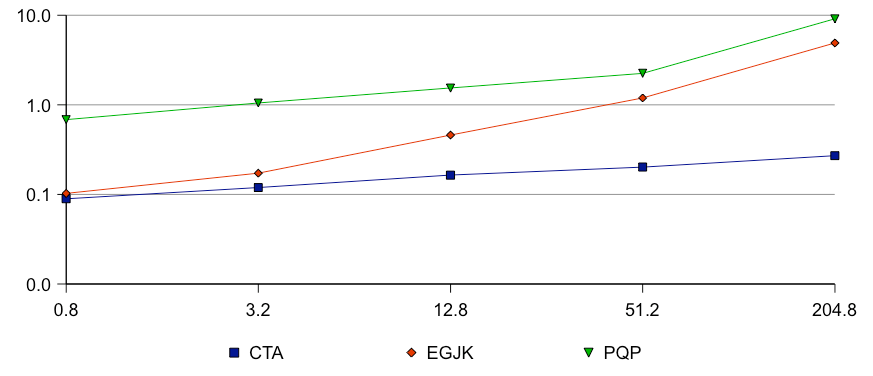
\includegraphics[width=\hsize]{Carpin_Figure_CTA.pdf}
    \mycaption{Time spend to solve a collision query as a function of
    the complexity of the involved polyhedra. The blue line outlines
    the performance of the proposed algorithm.}
    \label{fig:Carpin_pic1}
\end{center}
\end{figure}





\paragraph{Organization}

\begin{enumerate}
    \item 6th IEEE International Workshop on Robot Motion and  Control: program committee
          member
   \item IEEE 2006 International Conference  on Information Reuse  and
Integration: program committee member
\item PerMIS 2006: program committee member
   \item 6th international joint conference on autonomous agents and multiagent
          systems: program committee member
\item Robocup Federation: elected Executive Member for the 2007-2009 term
\item Organizer of  a tutorial on "USARSim/MOAST: Highly Realistic Simulation and Control for Multi Robot" held at the IEEE International
Conference on Robotics and Automation (Orlando-FL, May 2006)
\item Organizer of a tutorial on "USARSim and MOAST: Advanced Tools for High-Fidelity Simulation of Distributed Robot Systems "   held at the annual conference
of the American Association for Artificial Intelligence  (Boston-MA, July 2006)
\end{enumerate}

\paragraph{Collaborations}
\begin{enumerate}
    \item {\sl National Institute of Standards and Technology, USA}\\
          Dr. Steve Balakirski\\
          Organization of the Virtual League Competion and development of USARSim
    \item {\sl University of Pittsburgh, USA}\\
          Prof. Mike Lewis\\
          Organization of the Virtual League Competion
    \item {\sl University of Udine, Italy}\\
          Prof. Claudio Mirolo\\
          Development of Algorithms for Collision Detection
    \item {\sl University  of Padova, Italy}\\
          Prof. Enrico Pagello\\
          Development of Algorithms for Multi-Robot Motion Planning
\end{enumerate}



%\paragraph{Publications}

%\begin{description}
 % \item[Journals]
 \nocite{Carpin:IEEEPRO2006}\nocite{Carpin:ACTA2006}\nocite{Carpin:AR2006}

 % \item[Conference Proceedings]
  \nocite{Carpin:IAS2006}\nocite{Carpin:RS1}\nocite{Carpin:RS3}
  \nocite{Carpin:PerMIS2006b}\nocite{Carpin:PerMIS2006a}\nocite{Carpin:ICRA2006GM}
  \nocite{Carpin:ICRA2006BCMOMMT}
 % \item[Books/Collections]
   \nocite{Carpin:LNCS4123}
%\end{description}
%\end{document}
%%% Local Variables:
%%% mode: latex
%%% TeX-master: "report"
%%% End:


\shorttitle{Knowledge and Information Management Systems}
\subsection{Knowledge and Information Management Systems}


Today's information services are rapidly changing from statically served data to
information that is dynamically tailored to each individual user's current needs. This
information is fetched instantaneously from networked, distributed sources which
themselves change and evolve continually. At the same time, new representation formats
allow to discover and specify the internal and functional structure of information and
drive services that previously required (human) understanding. Technically, we observe the
convergence of databases, Internet, and distributed systems into semantically enriched
knowledge systems which allow the casual as well as the professional user to deal with the
ever-growing amount of information available.  Another issue is the presentation of
information to the user.  Data visualization is concerned with the management of large
data, the filtering and extraction of salient features, and their visual representation in
an expressive, intuitive, and interactive manner.

%%% Local Variables:
%%% mode: latex
%%% TeX-master: "report"
%%% End:

\newpage
\subsubsection{Reasoning, Semantics, and Knowledge  Management}
\label{ict:modeling:kohlhase} \index{Kohlhase, Michael}

\paragraph{Research Team}
Michael Kohlhase (Professor),
Heinrich Stamerjohanns (Head of CS Labs, see~\ref{ict:stamer}),
Christoph Lange (PhD Student),
Christine M\"uller (PhD Student),
Normen M\"uller (PhD Student),
Immanuel Normann (PhD Student),
Florian Rabe (PhD Student),
Andrea Kohlhase (Research Programmer) \\

%%% give a very short (150 words description of your research area)
%% Hint: this can be copied from the research areas document (../masterplan/research-areas)

The ability to represent knowledge about the world and to draw logical inferences is one
of the central components of intelligent behavior, as a consequence, reasoning components
of some form are at the heart of many artificial intelligence systems.

The work of the KWARC (\underline{K}no\underline{w}ledge \underline{A}daptation and
\underline{R}easoning for \underline{C}ontent) group centers around building knowledge
management systems for e-science applications, in particular for the natural and
mathematical sciences.  The main assumption in this work is that if the structure of the
factual content of scientific documents, their contributions and dependencies regarding a
larger knowledge context is made sufficiently explicit, then this structure becomes
amenable to machine manipulation. Thus high-level added-value (web)-services can be offered,
e.g. semantic search and navigation (independent of the surface presentation),
user-adaptive presentation and content tailoring, and extended semantic quality control up
to proof verification.

\paragraph{Highlights}

%%% give a short (500 words)description of the research highlights. 1 figure costs 100 words
The highlight in 2006 was the publication of a 500 page book on OMDoc in the Springer
Lecture Notes in Artificial Intelligence series~\cite{Kohlhase:omdoc1.2}. OMDoc
({\underline{O}}pen {\underline{M}}athematical {\underline{Doc}}uments) is an
{\sc{Xml}}-based representation format for mathematical knowledge developed in the KWARC
group. This format is used in various ($\geq 10$) international projects as the knowledge
representation base.

\begin{figure}[ht]
\begin{center}
  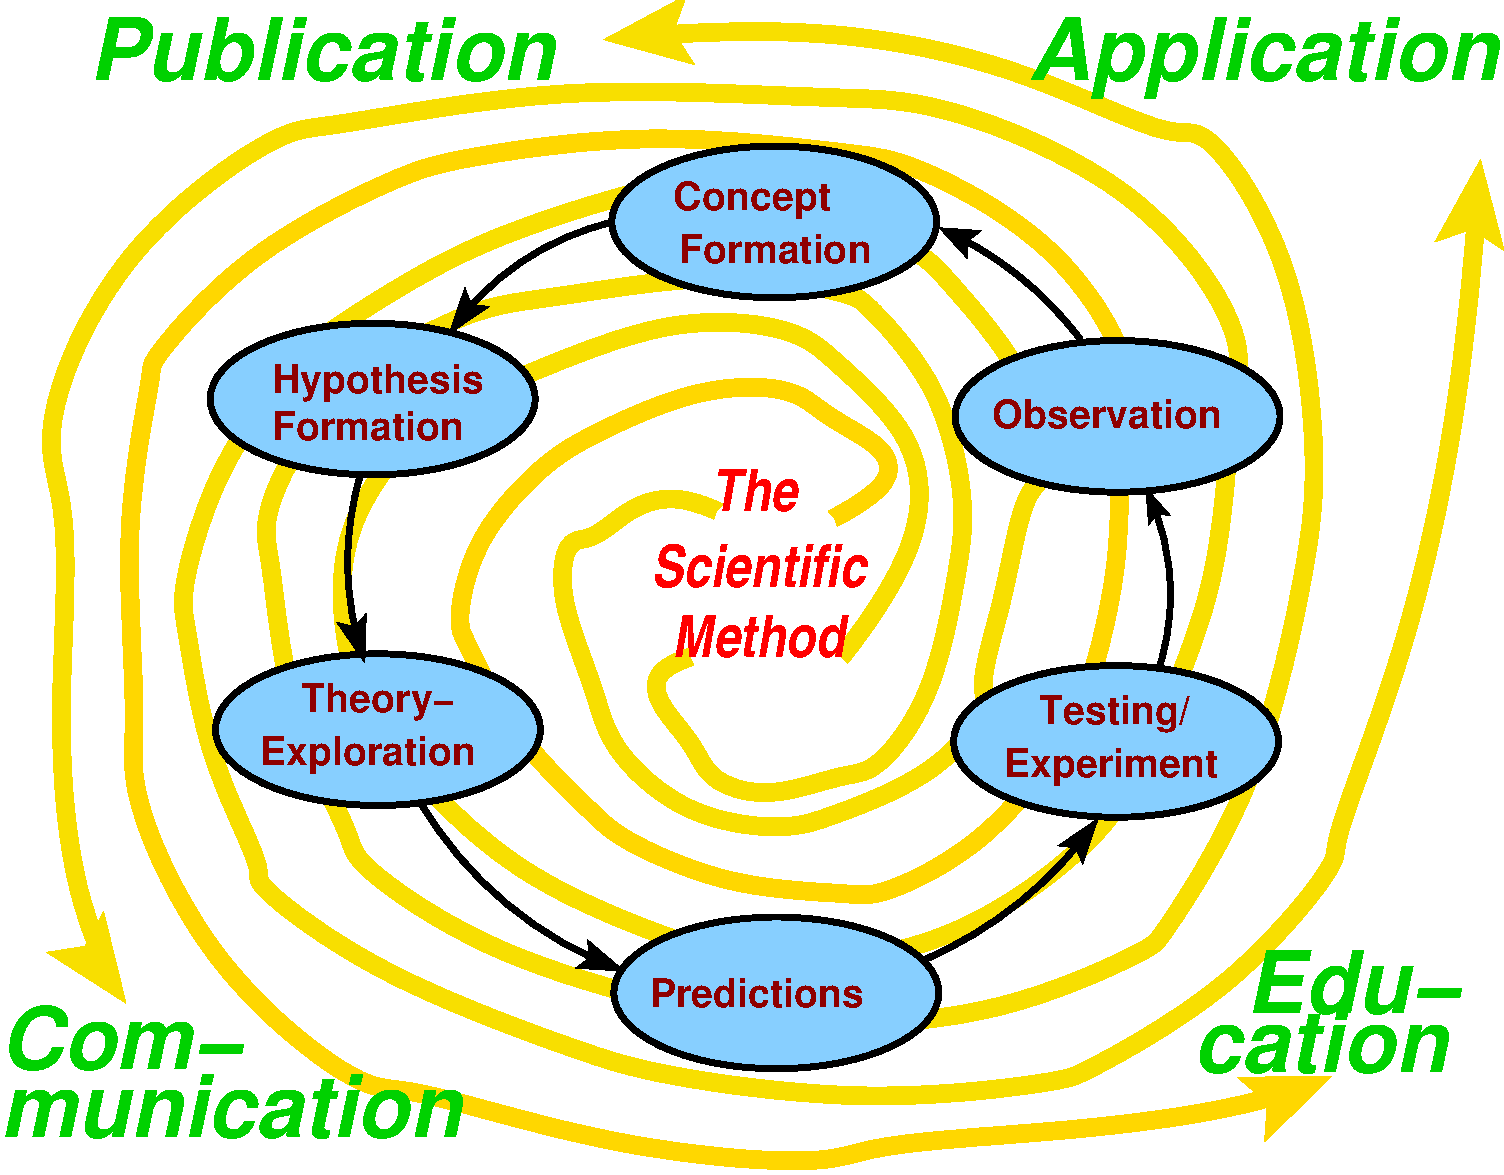
\includegraphics[width=7cm]{sci-method}
\end{center}
\caption{The Spiral View of Scientific Method}\label{fig:nw-Methode}
\end{figure}

We have extended the knowledge representation infrastructure in OMDoc to other topics in
the natural sciences to make it into a general semantic representation language that
supports seamless computer support in a ``{\emph{Scientific Semantic
    Web}}''~\cite{HilKohSta:copmem06}. Our starting point is the view of the
{\emph{scientific method}} as a spiral (Fig.~\ref{fig:nw-Methode}). In this view,
scientific research moves in a spiral trajectory from original ideas to results and
applications. At the moment, most of the steps in Fig.~\ref{fig:nw-Methode} are separately
supported by software systems, e.g. literature searches in Google Scholar or Wikipedia,
theory exploration in computer algebra systems and experiments in simulation systems. But
the systems are, largely, not able to inter-operate since they use differing data formats,
make differing model assumptions, and are bound to an implicitly given context that is
only documented in publications about the systems. A joint and universally applicable
representation language will be an enabling technology that alleviates these problems.

To make this vision come true, we have developed
\begin{enumerate}
\item a highly efficient, content-based document retrieval engine for
  mathematics~\cite{KohSuc:asemf06},
\item an OMDoc-based semantic WIKI~\cite{LanKoh:swim06,LanKoh:swmkm06,lange06:wikiblog},
\item a theoretical foundation for invasive editors and implementations in the MS Office
  suite~\cite{Kohlhase:UserAsPrisoner,Kohlhase:MediaOrMedeaSociety,Kohlhase:emPowerPoint},
\item methods for the discovery of theory morphisms in mathematical
  libraries~\cite{Normann:etrpti06}
\item a methodology for an ontology-based management of
  change~\cite{NRM:omdoc2vf06,Mueller06:locutor-lwa}, and
\item a representation format for logical systems with logic morphisms and
  proofs~\cite{rabe:dfol:06,rabe:moloss:06}
\end{enumerate}
We have started a research group of undergraduate CS students that undertake the
translation of the Cornell EPrint Archive from {\LaTeX} to XHTML+MathML (we can currently
translate 45\% of 400.000 articles in Physics, Mathematics, Computational Biology, and
Computer Science). This corpus will subjected of a semantic analysis with computational
linguistics methods and will be the basis of scalability studies for the methods and
representation formats presented above.

\paragraph{Organization}

In 2006, Prof. Michael Kohlhase was
\begin{enumerate}
\item Program and Conference Co-Chair of the 29.th Annual German Conference on Artificial
  Intelligence KI'06\cite{KI06}
\item Trustee of the Conference on Automated Deduction
\item Trustee of the Mathematical Knowledge Management Interest Group
\item Trustee of the CALCULEMUS Interest Group
\item Member of the Executive Committee of the OpenMath Society
\item Member of the MathML Working Group of the World Wide Web Consortium (W3C)
\item Member of 11 Program Committees of International Conferences.
\item Member of the Reviewer's College of the Engineering and Physical Sciences Review
  Research Council (EPSRC)
\item General Editor ``QPQ: an Online Journal for Peer-Reviewed Deductive Software
  Components'' {\url{http://www.qpq.org}}
\item Editor ``Journal of Applied Logic'', Elsevier.
\item Member of the ``Auswahlausschu\ss der Studienstiftung des Deutschen Volkes''
\end{enumerate}

\paragraph{Collaborations}
Prof. Michael Kohlhase is a Vice Director of the ``Safe and Secure Cognitive Systems'' of
the newly founded Department of the German Research Institute Lab Bremen. This leads to an
intensive collaboration of the KWARC group with this research group, which includes joint
projects and supervision of students. Further collaborations of the KWARC group include
\begin{enumerate}
    \item {\sl Rice University, USA}\\
          Prof. Richard Baraniuk\\
          Extending the Connexions Representation Format CNXML
    \item {\sl National Institute of Standards, USA}\\
          Dr. Bruce Miller\\
          Transforming {\LaTeX} documents to OMDoc/CNXML
    \item {\sl International University Bremen}\\
          Prof. Peter Baumann\\
          Extending OMDoc to GIS-Data/Living Documents
    \item {\sl Institute for Science Networking}\\
          Prof. Eberhard R. Hilf\\
          Extending OMDoc to PhysML
    \item {\sl Carnegie Mellon University, USA}\\
          Prof. Frank Pfenning, Prof. Peter Andrews\\
          Higher-Order Theorem Proving and Meta-Logical Frameworks
    \item {\sl Universit\"at des Saarlandes}\\
          Prof. J\"org Siekmann, Dr. Christoph Benzm\"uller\\
          Higher-Order Theorem Proving
    \item {\sl Deusches Forschungszentrum f\"ur K\"unstliche Intelligenz, Saarbr\"ucken}\\
          Dr. Dieter Hutter\\
          Ontology-based Management of Change
    \item {\sl Design Science Inc.}\\
          Dr. Robert Miner\\
          Mathematical Document Retrieval
\end{enumerate}

% \paragraph{Awards, Prizes}
% % list the awards, prizes you have received in 2005, if none have been received, plese delete this
% % subsection.
% \begin{enumerate}
% \item DAAD, grant for a year at Carnegie Mellon University.
% \end{enumerate}

\paragraph{Grants}
% list the running grants in 2005, if none have been received, please delete this
% subsection.
\begin{enumerate}
\item Funded by EU-IST (FP 6), \emph{ ONCE-CS}, (July 2005 -
December 2007)
\\
\item Funded by EU-IST (FP 6) \emph{JEM}, (July 2006 - July 2009)

%\item Industry: Design Science Inc. Grant for transforming Cornell Eprint archive.
\end{enumerate}

%\paragraph{Publications}
\nocite{BenBroKoh:csil06}
%\end{document}
%%% Local Variables:
%%% mode: latex
%%% TeX-master: "report"
%%% End:

% LocalWords:  Stamerjohanns EECS uller Normen Normann Rabe KWARC daptation Xml
% LocalWords:  easoning ontent OMDoc athematical uments Google Baraniuk CNXML
% LocalWords:  Baumann GIS Hilf Pfenning Universit des Saarlandes org Siekmann
% LocalWords:  Benzm Krieg uckner Deusches


\subsubsection{Simulation and Control of Complex Dynamical Systems}\label{ict:modeling:antoulas}
\index{Antoulas, A.C.}

\paragraph{Research Team}
Athanosios Antoulas (Professor)

Model reduction seeks to replace a large-scale system of differential
or difference equations (the outcome of discretizing a PDE, perhaps) by a
system of substantially lower dimension, that ideally, has the same
response characteristics as the original system,
yet requires far less computational resources for realization than the
potentially unmanageable levels that may be required by the larger original
system.

Two main currents can be identified among methodologies for model reduction.
Balanced approximation methods are built upon a family of
ideas with very close connection to the singular value decomposition.
These methods preserve stability and allow for global error bounds but
often do not scale well in terms of
computational efficiency and stability when applied to large scale problems.
Moment matching methods are based principally on Pad\'e-like
approximations and for large-scale problems have lead naturally to the
use of Krylov and rational Krylov subspace methods. These methods generally
enjoy greater efficiency  and numerical stability.
A strong current trend aims at combining these two approaches by deriving
iterative methods which achieve approximate balanced reduction.

\paragraph{Highlights}

%%% give a short (500 words)description of the research highlights. 1 figure costs 100 words

% to include a figure, generate a file xxx.pdf and integrate the following lines
%% \begin{figure}[ht]
%%   \begin{center}
%%     \includegraphics[width=10cm]{xxx}
%%     \caption{The caption of the figure}
%%     \label{fig:xxx}
%%   \end{center}
%% \end{figure}
% to reference it use ``Figure.~\ref{fig:xxx}''; the numbers will be computed automatically.

Our research activities are concerned with the circle of ideas surrounding
model reduction. It provides efficient
and robust methods for producing reduced order models of
large state space systems.  These activities
have an impact both in system theory of complex systems
as well as in applied mathematics and in particular numerical methods for
large-scale problems.  Once the theory and computational
methods are developed, we expect that high quality software will result and
have applications in many areas of engineering.
This will enable at a later stage,
the design of real time controllers for complex systems.

{\it Broader impact resulting from the proposed activities}.
In today's technological world, physical processes are
described mainly by mathematical models, which are used to
simulate the behavior of the physical processes in question.
Sometimes, they are also used to modify or control their behavior.
In this framework, there is an ever increasing need for
improved accuracy which leads to models of high complexity.

The basic motivation for system approximation is the need in many
instances for a simplified model of a dynamical system, which
however captures the main features of the original complex model.
This need arises from limited computational, accuracy, and storage
capabilities. The simplified model is then used in place of the
original complex model, either for {\it simulation}, or {\it control}.

Important areas of application of model reduction are: VLSI
(Very Large Scale Integration) design, weather prediction,
air quality management, molecular dynamics simulations, simulation and
control of chemical (e.g. CVD - Chemical Vapor Deposition) reactors,
car windscreen quality management, simulation and control of MEMS (Micro
Electro Mechanical Systems) devices, e.g. micromirrors, to name but a few.
Thus the proposed activities have potential benefits for society at large.

%\paragraph{Organization}
% list the (research) events you have organized, if any,

%\begin{enumerate}
%\item  ....
%\item   ...
%\item  ...
%\end{enumerate}

%\paragraph{Collaborations}
%\begin{enumerate}
%\item ...
%\item ...
%\item ...
%\end{enumerate}

\paragraph{Grants at RICE University}
% list the running grants in 2005, if none have been received, please delete this
% subsection.
\begin{enumerate}
\item
Funded by US National Science Foundation, R38570-776000, NSF CCR-0306503, \emph {Model
  Reduction for Structured Dynamical Systems}, (August 2003 - July 2006)
% Amount: \$$436,607.00$ 

\item
Funded by US National Science Foundation,  ITR (Information Technology Research) Grant,
collaborative with Purdue and Florida State, R38670-776000, NSF ACI-0325081, \emph
{Research on Model Reduction of Dynamical Systems for Real-time Control}, (January 2003 -
August 2007)
      %Amount: \$$1,826,959.00$\\

\item
Funded by US National Science Foundation, OSR No.: 06052204, NSF CCF-0634902,
\emph{Advanced Projection Techniques for Dimension Reduction of Large Scale Dynamical
  Systems}, (October 2006 - September 2009)

\end{enumerate}

%\paragraph{Patents}
% list the grants you have received in 2005, if none have been received, plese delete this
% subsection.
%\begin{enumerate}
%\item
%\item
%\end{enumerate}


%\paragraph{Awards, Prices}
% list the grants you have received in 2005, if none have been received, plese delete this
% subsection.
%\begin{enumerate}
%\item
%\item
%\end{enumerate}

%\paragraph{Publications}
% list the publications of 2005 (also accepted and in press), if none have been received, plese delete this
% subsection. Enter the publications into the SES publications database at
% http://kwarc.eecs.iu-bremen.de/ses-pubs/index.php and only reference them here.
\nocite{aca1}

% \begin{description}
% \item[Book]
% A.C. Antoulas,
% ``Approximation of large-scale dynamical systems'',
% Book Series: {\it Advances in Design and Control} {\bf DC 06}, 479 pages,
% SIAM, Philadelpia (2005).
% \item[Journal Paper]
% D.C. Sorensen and A.C. Antoulas,
% {\it On model reduction of structured systems}, in
% "Dimension Reduction of Large-Scale Systems",
% Edited by P. Benner, V, Mehrmann and D.C. Sorensen,
% Springer Verlag, pages 125-138, (2005).
% \item A.C. Antoulas, {\it A new result on passivity preserving
% model reduction}, Systems and Control Letters,
% Volume 54, Issue 4, Pages 361-374, April (2005).
% \item[Journal Paper]
% S. Gugercin and A.C. Antoulas,
% {\it Model reduction of large-scale systems by least squares},
% Linear Algebra and Applications,
% Special Issue on Order Reduction of Large-Scale Systems,
% Edited by P. Benner, D.C. Sorensen, R. Freund, and A. Varga, accepted
% for publication, 2005.
% \item[Journal Paper]
% A.C. Antoulas, {\it Frequency domain representation and singular
% value decomposition}, UNESCO EOLSS (Encyclopedia for the Life Sciences),
% Contribution 6.43.13.4, 52 pages, in press, 2005.
% \item[Journal Paper]
% A.C. Antoulas, {\it An overview of model reduction methods for large-scale
% dynamical systems}, IFAC Annual Reviews in Control, Invited Paper,
% JARAP vol. {\bf 228} (2005).
% \item[Report]
% Q. Zhou, K. Mohanram, and A.C. Antoulas,
% {\it Structure Preserving Reduction of Frequency-dependent Interconnect},
% Technical Report, June (2005).
% \item[Journal Paper]
% A.C. Antoulas, E. Gildin, R.H. Bishop and D.C. Sorensen,
% {\it Model and controller reduction for seismically excited buildings},
% submitted to "Structural Control and Monitoring", November (2005).
% \item[Journal Paper]
% S. Gugercin, A.C. Antoulas, and C. Beattie, Technical Report,
% {\it An iterative rational Krylov approach to optimal H2 model reduction},
% SIMAX (SIAM J. Matrix Analysis and Applications), 2006 (submitted).
% \item[Journal Paper]
% A.J. Mayo and A.C. Antoulas,
% {\it A framework for the general realization problem},
% {Linear Algebra and Its Applications}, Special Issue in honor of P.A. Fuhrmann,
% Edited by A.C. Antoulas, U. Helmke, J. Rosenthal, V. Vinnikov, and E. Zerz.
% 2006 (sumbitted).
% \item[Journal Paper]
% S. Gugercin, A.C. Antoulas, and C.A. Beattie,
% {\it Krylov-based controller reduction for large-scale systems},
% {Automatica}, 2006 (submitted).
%\end{description}
%%\end{document}
%%% Local Variables:
%%% mode: latex
%%% TeX-master: "report"
%%% End:

\subsubsection{Raster Data Services}
\index{Baumann, Peter}
\paragraph{Research Team}
Peter Baumann (Professor), Angelica Garcia Gutierrez (PhD Student)\\

Raster data occur in various dimensions, be they observed phenomena or generated data
sets. Examples comprise satellite imagery and mapping, geo physics and exploration,
medical imagery, engineering data, and statistics data. A key property they have in common
is their extreme volumes, often Giga- to Petabyte per object.

With the advent of sufficiently large disk capacities data providers more and more tend to
publish such large Multidimensional Discrete Data (MDD) - GoogleEarth is a prominent
example. Generally such services are implemented in an ad-hoc manner, and consequently
offer limited functionality (such as GoogleEarth: zoom and pan on satellite
maps). However, flexible, value-added data navigation and analysis requires more, both for
experts (such as exploration engineers) and the general public (where internally complex
functionality like local weather prediction obviously should be wrapped for easy access).

MDD database and Web service support raises new questions on all levels: conceptually,
formal models are needed to describe data and services; query languages resp. request
interfaces need to be designed based on these foundations. Efficient implementation,
including optimizing query evaluation and storage structures, is needed. The high volume
suggests to include tape robots as nearline storage facilities. Last but not least
services for as many application domains as possible need to be realized to gain domain
understanding and to evaluate service implementations.

In our research we investigate on the principles of MDD management based on the rasdaman
("raster data manager") system acting as a research platform. Application domains
inspected are mainly stemming from earth system research, such as 2-D to 4-D remote
sensing, exploration, marine, and climate data. As a byproduct we are actively engaged in
the Open GeoSpatial Consortium where we contribute to the standardization of geo raster
services.

\paragraph{Highlights}

An important work package is contribution to geo raster service
standardization in the Open GeoSpatial Consortium (OGC,
\url{http://www.opengis.org}). We are actively contributing in the
Web Coverage Service (WCS) Revision Working Group where the
substantially revised WCS version 1.1 has been finished by the end
of 2006. Based on the experience gained there and the WCS
shortcomings spotted we have propose the concept of a Web Coverage
Processing Service (WCPS); Figure~\ref{fig:ndvi} exemplifies usage
of WCPS by dynamically deriving the NDVI of a Landsat satellite
scene; the NDVI I of an image is defined as I=(nir-red)/(nir+red),
in the right image it is thresholded as $I>0.6$. In June 2006, WCPS
has been lifted to a Best Practice Paper (which implies OGC
endorsement), it is estimated that WCPS can become a Draft Standard
end of 2006 / beginning of 2007, and a full standard by summer 2007.
Several institutions, among them German mapping (AdV) and
geophysical institutions (such as BGR) have expressed their
interest.

In parallel to the conceptual work on WCS and WCPS, our group implements both
services. Prototypes have been demonstrated at various occasions in 2006, among them OGC
Technical Commitee meetings. For 2007 it is planned to set up large-scale services fo
thorough evaluation prior to freezing the final standard document.

The GALEON (Geo-interface to Atmosphere, Land, Earth, Ocean, NetCDF) project launched in
2005 meantime has become an OGCnetwork (\url{http://www.ogcnetwork.net/galeon}); besides
contributing to WCS requirements it is starting now to hands-on evaluate the new WCS
1.1. IUB will contribute our WCS implementation, which is under work,

As part of the IRCCM project (\url{http://www.irccm.org}) and in collaboration with IUB's geo group and
AWI Bremerhaven, a standards-based open service for marine research data has been set up
which combines bathymetry data and video mosaics acquired by a French underwater
robot. Data describe an underwater volcano in the Norwegian Atlantic area known as
Hakon-Mosby. This service is the first step towards a more comprehensive multi-sensor
fusion service between IUB and AWI.

For the ICSU CODATA (Committee on Data in Science and Technology) a German section has
been established as an "e.V." and has been accredited with CODATA International. As a side
effect of this work, several fruitful research contacts have emerged, such as with the
Chinese Academy of Science (see above).

\begin{figure}[ht]
  \begin{center}
     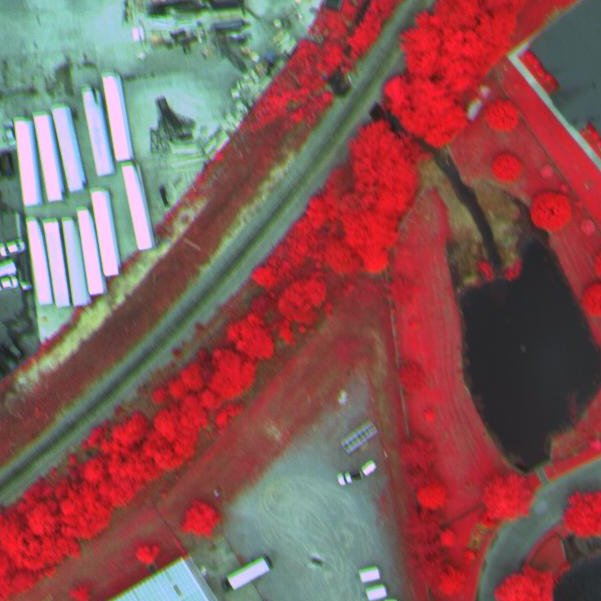
\includegraphics[width=3.5cm]{ndvi-1.jpg}
     
\includegraphics[width=3.5cm]{ndvi-2.jpg}
    \caption{The Normalized Difference Vegetation Index (NDVI) as a database / Web
      service query (rasdaman screen shots).}\label{fig:ndvi}
   \end{center}
\end{figure}

\paragraph{Collaborations}

In 2006 several new international research cooperations have been established:
\begin{enumerate}
\item {\sl Universidade de Campinas (Unicamp), Campinas, Brazil}

  Prof. Claudia Bauzer Medeiros is Head of the Laboratory of Information Systems (LIS) at
  the Institute of Computing, UniCamp, and President of the Brazilian Computer
  Society. With her group she works on advanced Web-based geo services with emphasis on
  agrocultural and environmental applications; to this end there is a long-standing
  relation with the Brazilian Ministry of Agriculture.

  In the collaboration, for which a joint research proposal has been submitted to
  DAAD/Germany and INPe/Brazil, both partners plan to extend Unicamp's geo services with
  IUB's raster services, based on the open OGC standards. The resulting system will be
  exercised in real life operation. Evaluation results will be brought into OGC to give
  feedback to the standards developers.

\item {\sl Universidad de Sinaloa, Sinaloa, Mexico}

  Dr. Ines Fernando Lopez Vega, who in 2004 has received his PhD from University of
  Arizona at Tucson, is building up his research on image time series
  evaluation. Collaboration is foreseen combining his interests with our raster service
  research and Michael Kohlhase's work on Semantic Web services.

  Collaboration was initiated in Fall 2006 with a visit of Dr Lopez Vega in the course of
  his co-supervision of Angelica Garcia Gutierrez's PhD work.

\item {\sl Chinese Academy of Sciences and Jilin University, Changchun, China}

  Prof. Liu Chuang plays an important role in China when it comes to provision and
  exploration of remote sensing data. Among others, she is Vice Director of the Institute
  of Geography and Natural Resources (IGNR) and director of the Spatial Data Commission,
  the Chinese Association of Geographic Information System (CAGIS), and Secretary General
  of a Working Group of Remote Sensing and Data Information Systems (RS/DIS).

  IUB, IGNR und Jilin University plan joint activities in the field of open
  standards-based geo services on high-volume in situ and remote sensing data, based on
  rasdaman. As a real life application IGNR's 100+ TB data archive of Chinese satellite
  imagery collected over several years will serve, today stored in hundreds of DVDs,
  unavailable to the researcher community. The Chinese National Disaster Reduction Center
  will be one of the first users, with application scenarions being river floods and
  earthquakes.
\end{enumerate}


Several tutorials have been given on the topic of raster services:
\begin{enumerate}
\item CODATA 2006 Conference, Beijing (3 hrs)
\item 1st International Symposium on Cooperation and Promotion of Information Resources in
  Science and Technology (under the auspices of the Chinese Ministry of Science and
  Technology), Beijing (2 hrs)
\item 19th IFIP World Computer Congress, Santiago de Chile (3 hrs)
\end{enumerate}

%\paragraph{Publications}

%\begin{description}
\nocite{PB:comogis,PB:codata,PB:fig}
%\end{description}
%%% Local Variables:
%%% mode: latex
%%% TeX-master: "report"
%%% End:

%\svnInfo $Id$
%\svnKeyword $HeadURL$

%\documentclass{article}
%\usepackage{epsfig}
%\begin{document}

\subsubsection{Visualization and Computer Graphics}
\index{Linsen, Lars}

\paragraph{Research Team}
Lars Linsen (Professor),
Sherin Al-Shbat (PhD Student),
Tetyana Ivanovska (PhD Student),
Tran Van Long (PhD Student),
Paul Rosenthal (PhD Student)\\

The Visualization and Computer Graphics Laboratory (VGCL) led by Prof.~Lars Linsen is
mainly concerned with topics from scientific and information visualization plus some
selected topics from computer graphics and geometric modeling.

Visualization is an inherently interdisciplinary field with application in many different
areas.  Scientific visualization deals with the visualization of data with spatial
interpretation such as computer-generated data from numerical simulations (physics,
chemistry) or measured data using scanning or sensoring techniques (medicine, life
sciences, geosciences).  The group's efforts are to generate visualization methods that
can handle large data sets efficiently, filter distinct features automatically or
interactively, and display the relevant information in a comprehensive and intuitive
fashion.  The research focuses on segmentation and isosurface extraction, hierarchical
methods, multi-variate data visualization, flow and tensor field visualization, and user
interaction.

Information visualization deals with the visualization of abstract data with no spatial
interpretation such as graph- or network-based data (life sciences, social sciences) or
multi-dimensional data (databases, ecomomics).  The group's efforts focus on interactive
exploration and analysis tools for such abstract data.

In the areas of computer graphics and geometric modeling the group's interest lies in
point-based methods, multi-resolution surface representation, and curves on surfaces.


\paragraph{Highlights} \ \\

{\em Direct Isosurface Extraction from Scattered Volume Data.}
Isosurface extraction is a standard visualization method for scalar volume data and has
been subject to research for decades.  Nevertheless, no isosurface extraction method
existed that directly extracts surfaces from scattered volume data without 3D mesh
generation or reconstruction over a structured grid. We have developed a method based on
spatial domain partitioning using a $k$d-tree and an indexing scheme for efficient
neighbor search. Our approach consists of a geometry extraction and a rendering step. The
geometry extraction step computes points on the isosurface by linearly interpolating
between neighboring pairs of samples. The neighbor information is retrieved by
partitioning the 3D domain into cells using a $k$d-tree. The cells are merely described by
their index and bitwise index operations allow for a fast determination of potential
neighbors. The final rendering step uses point-based rendering techniques.

\begin{figure}[ht]
  \begin{center}
    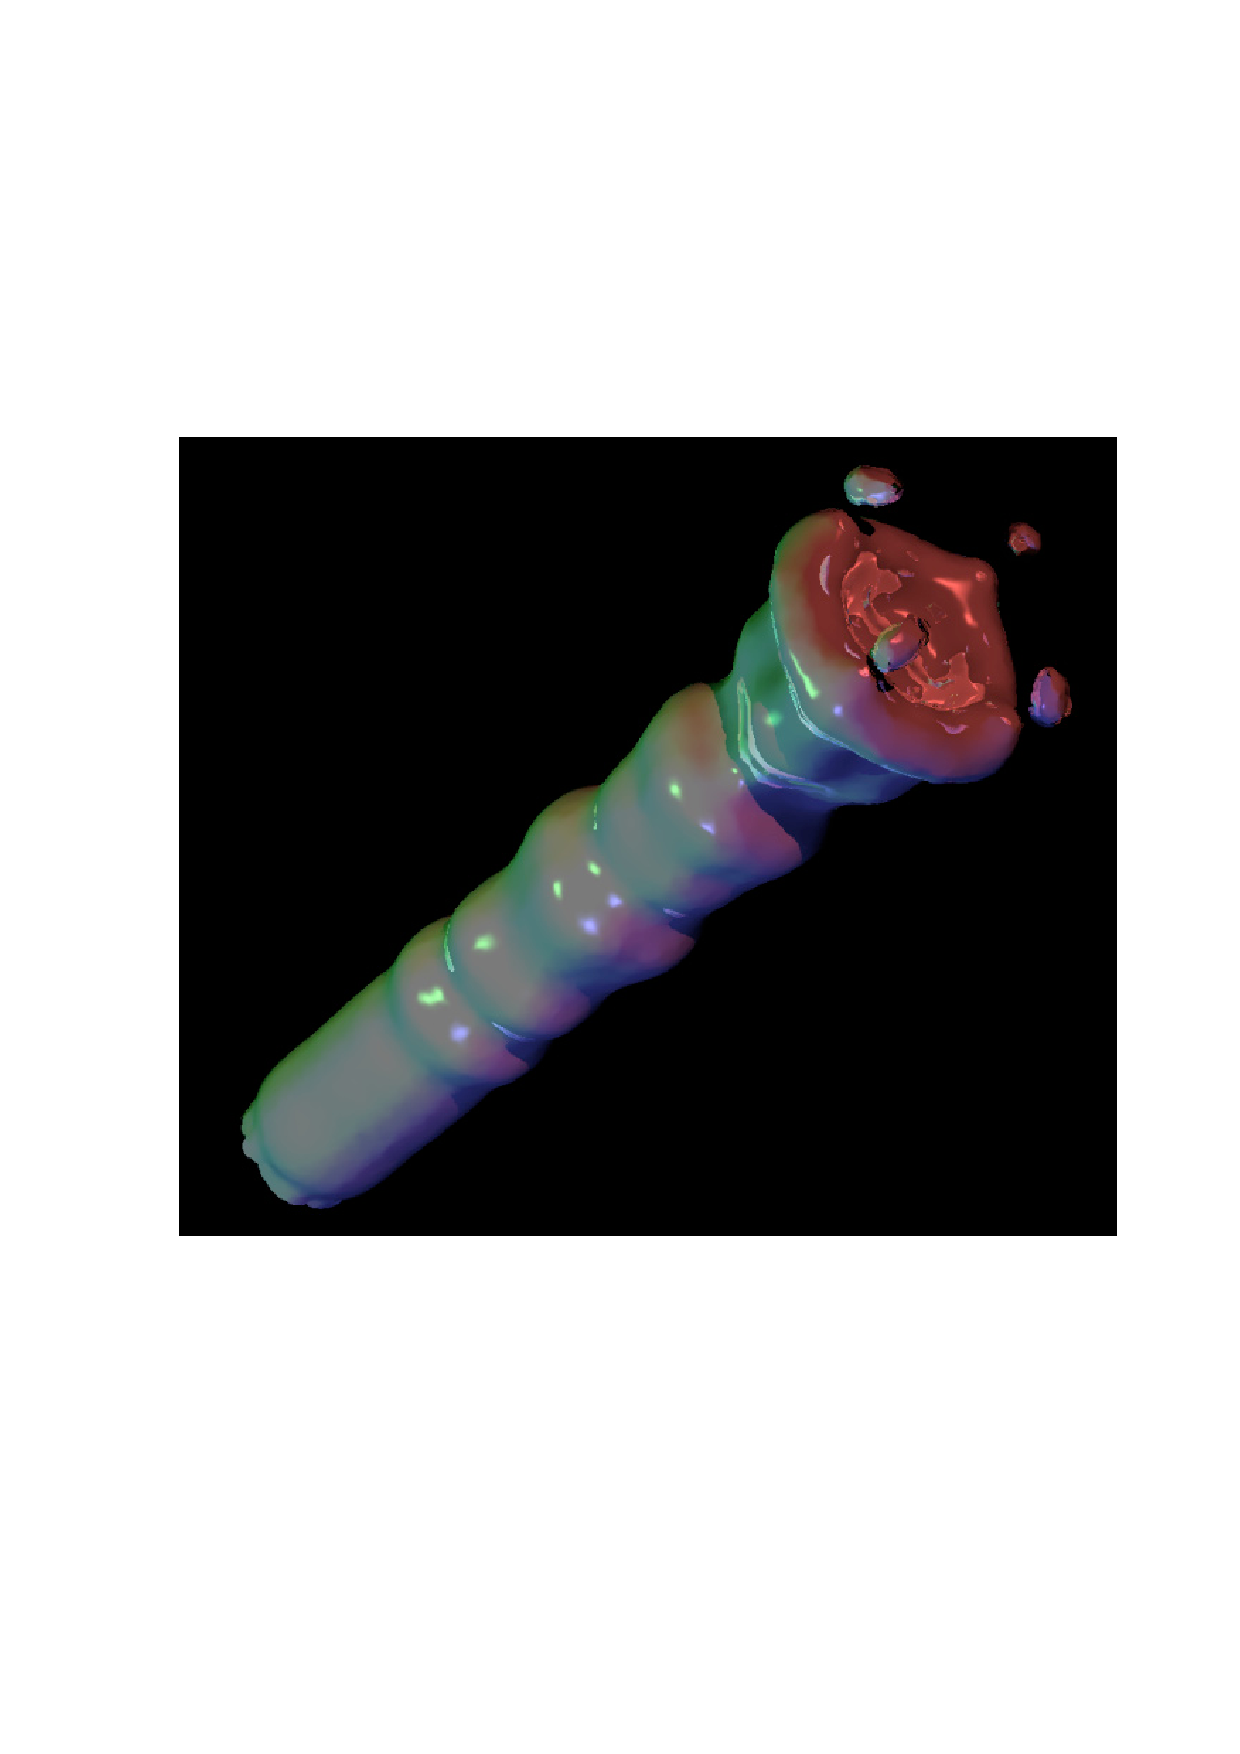
\includegraphics[width=\hsize]{Linsen_2006_Fig1.pdf}
    \caption{Point-based ray tracing of isosurface directly extracted from a scattered
      volume data. The scattered data set is a uniform random sampling of simulation data
      of fuel injection into a combustion chamber.}
    % \caption{Point-based ray tracing of isosurface directly extracted from a scattered
    %   volume data. The scattered data set is a uniform random sampling of simulation
    %   data of fuel injection into a combustion chamber.}
    % \label{fig:profxxx}
   \end{center}
\end{figure}

\noindent
{\em Using Ray Intersection for Dual Isosurfacing.}
Isosurface extraction using dual contouring approaches have been developed to generate a
surface that is dual in terms of the underlying extraction procedure used when compared to
the standard Marching Cubes (MC) method. These approaches address some shortcomings of the
MC methods including feature-detection within a cell and better triangles. We have
developed a simple method based on the MC method and the ray intersection technique to
compute isosurface points in the cell interior. One of the advantages of our method is
that it does not require Hermite data, i.e., the discrete scalar values at vertices
suffice. We compute ray intersections to determine isosurface points in the interior of
each cell, and then performed a complete analysis of all possible configurations to
generate a look-up table for all configurations.  We use a look-up table to optimize the
ray intersection method to obtain minimum number of points necessarily sufficient for
defining topologically correct isosurfaces in all possible configurations.

\noindent
{\em Structure-accentuating Dense Flow Visualization.}
Vector field visualization approaches can broadly be categorized into approaches that
directly visualize local or integrated flow and approaches that analyze the topological
structure and visualize extracted features. Our goal was to come up with a method that
falls into the first category, yet reveals structural information. We have developed a
dense flow visualization method that shows the overall flow behavior while accentuating
structural information without performing a topological analysis. A flow integration step
generates a density field by tracing particles under the influence of the underlying
vector field. The resulting density is high in attracting regions and low in repelling
regions. Density is measured by the number of particles per region accumulated over
time. The density fields for forward and backward propagation are explored using
texture-based rendering techniques.  We obtained dense flow visualizations that display
the overall flow behavior, emphasize critical and separating regions, and indicate flow
direction in the neighborhood of these regions.

\begin{figure}[ht]
  \begin{center}
     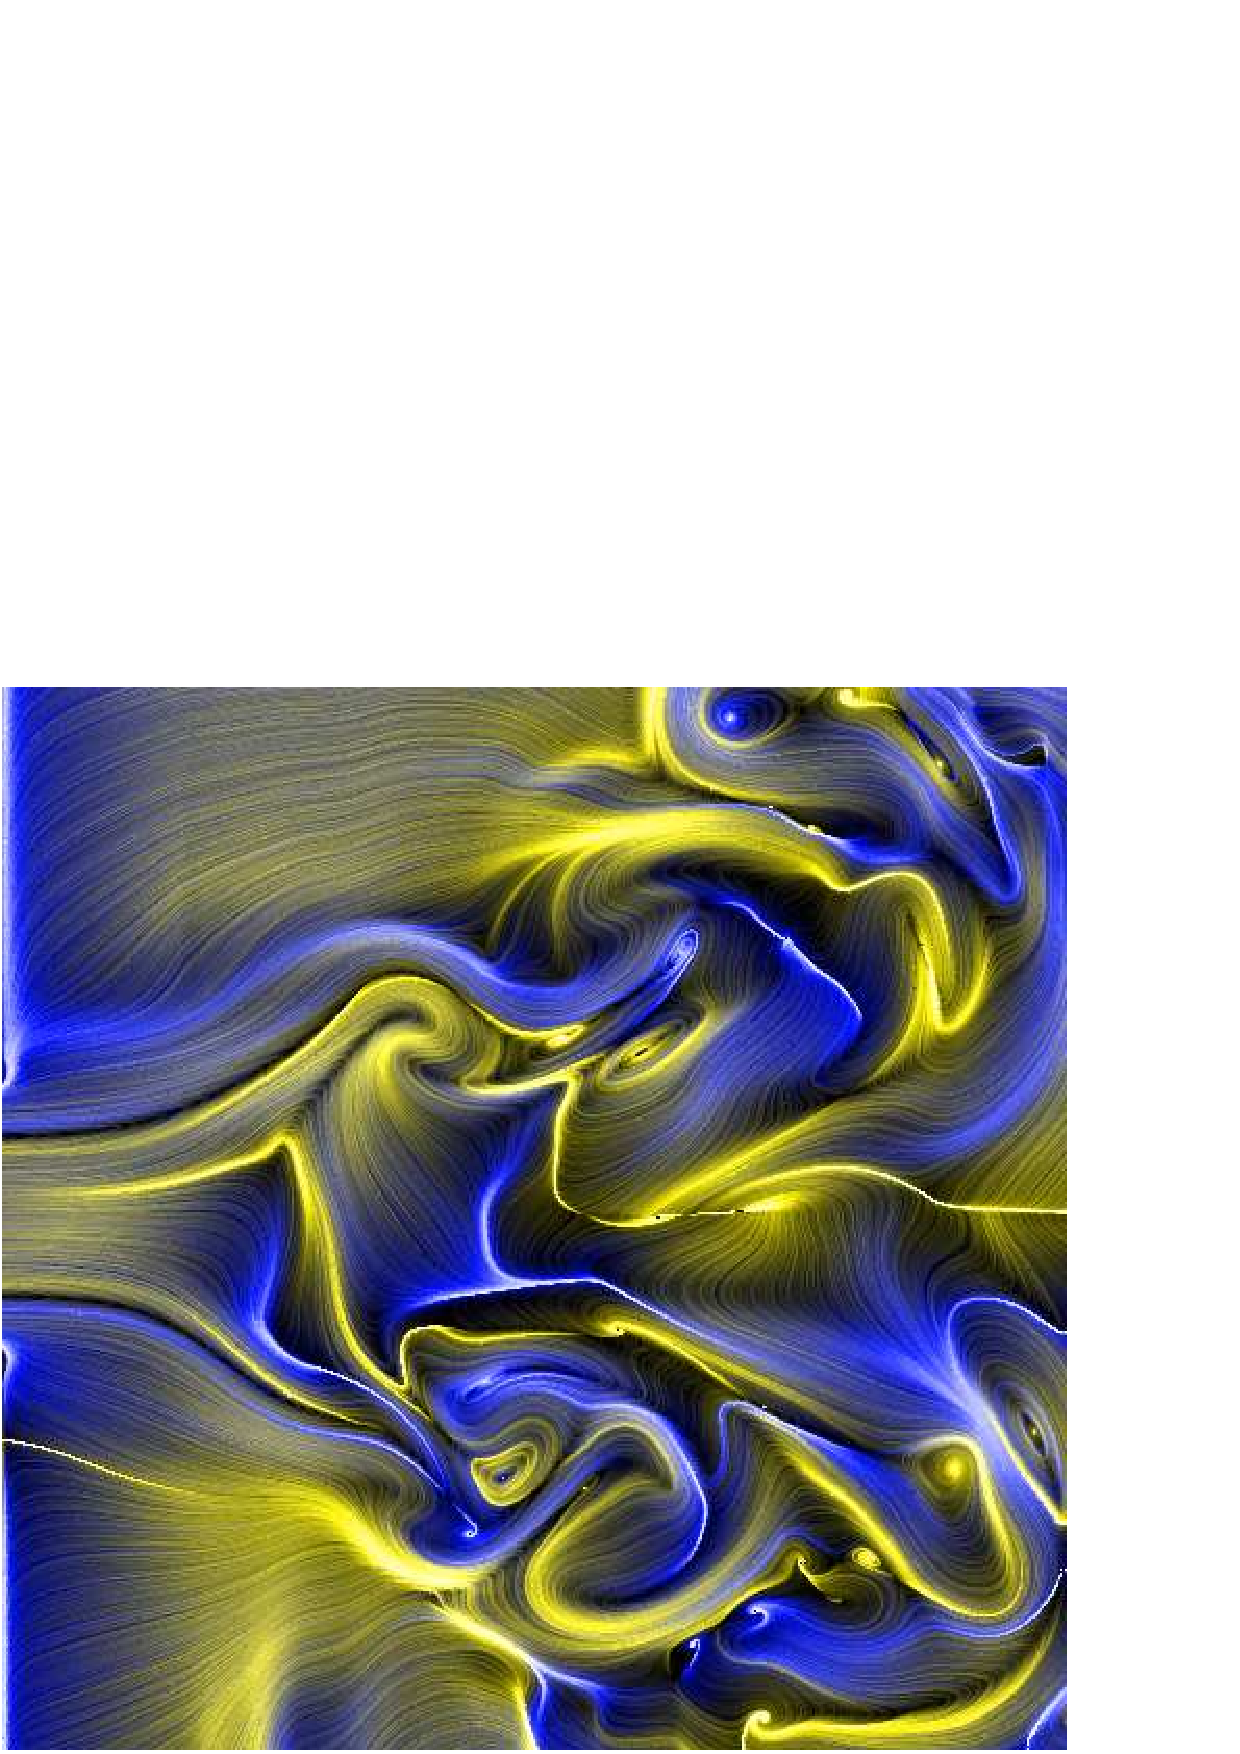
\includegraphics[width=\hsize]{Linsen_2006_Fig2.pdf}
    \caption{Structure-accentuating dense flow visualization applied to 2D simulation of
      a swirling jet.}
    %\caption{Structure-accentuating dense flow visualization applied to 2D simulation of a swirling jet.}
     % \label{fig:profxxx}
   \end{center}
\end{figure}

\noindent
{\em Visual Analysis of Gel-free Proteome Data.}
We developed a visual exploration system supporting protein analysis when using gel-free
data acquisition methods. The data to be analyzed is obtained by coupling liquid
chromatography (LC) with mass spectrometry (MS). LC-MS data has the properties of being
non-equidistantly distributed in the time dimension (measured by LC) and being scattered
in the mass-to-charge ratio dimension (measured by MS).  A hierarchical data
representation and visualization method is used for large LC-MS data. Based on this
visualization we have developed a tool that supports various data analysis steps like
deisotoping, landmark-based registration, and differential protein expression
analysis. Our visual tool provides a global understanding of the data, intuitive detection
and classification of experimental errors, and extensions to LC-MS/MS, LC/LC-MS, and
LC/LC-MS/MS data analysis.


\paragraph{Organization}
% list the (research) events you have organized, if any,

\begin{enumerate}
\item International conference on {\em Visualization in Medicine and Life Sciences (VMLS
    06)} held July 19--21, 2006, at Binz, R{\"u}gen, Germany
  (http://www.lars-linsen.de/vmls).  Organizers: Lars Linsen, Hans Hagen (University of
  Kaiserslautern), and Bernd Hamann (University of california, Davis).
\end{enumerate}

\paragraph{Collaborations}
\begin{enumerate}
\item {\sl Institut f{\"u}r Mathematik und Informatik, Ernst-Moritz-Arndt-Universit{\"a}t Greifswald, Germany}.\\
  Prof.~Georg F{\"u}llen, Julia L{\"o}cherbach, Steffen Rudnick.\\
  (1) Visualization of protein-protein interaction. \\
  (2) Visualization of gel-free proteomics data.\\
  (3) Simulation and animation of urban tree growth.
\item {\sl Institut f\"ur Mikrobiologie, Ernst-Moritz-Arndt-Universit\"at
    Greifswald, Germany}. \\
  Prof.~Michael Hecker, Dr.~J{\"o}rg Bernhardt, Dr.~D{\"o}rte Becher.\\
  Visualization of gel-free proteomics data.
\item {\sl Decodon GmbH, Greifswald, Germany}. \\
  Dr.~Matthias Berth, Dr.~J{\"o}rg Bernhardt.\\
  Visualization of gel-free proteomics data.
\item {\sl Institut f\"ur Diagnostische Radiologie und Neuroradiologie,
    Ernst-Moritz-Arndt-Universit\"at
    Greifswald, Germany}. \\
  Prof.~Norbert Hosten, Dr.~S{\"o}nke Langner, Martin Domin. \\
  Glyph- and tracking-based visualization of diffusion MRT data.
\item {\sl Poliklinik f\"ur zahn\"arztliche Prothetik und Werkstoffkunde,
    Ernst-Moritz-Arndt-Universit\"at
    Greifswald, Germany}. \\
  Prof.~Bernd Korda{\ss}.\\
  Virtual placement and interactive optimization for functional occlusion in
  prosthodontics.
\item {\sl Institut f\"ur Psychologie, Ernst-Moritz-Arndt-Universit\"at
    Greifswald, Germany}. \\
  Prof.~Klaus Landwehr.\\
  An interactive system for the generation of symmetric images with respct to symmetry
  groups.
\item {\sl Fraunhofer-Institut f\"ur Produktionstechnologie, Aachen, Germany}. \\
  Prof.~Christian Brecher, Prof.~Fritz Klocke, Lothar Glasmacher, Dr.~Olaf Dambon, Richard Zunke, Timo Wenzel.\\
  MoldFinish: Intelligent polishing system for automated finishing in tool and mold
  making.
  % (1) MoldFinish: Intelligents Poliersystem zur Automatisierung und Endbearbeitung im Werkzeug- und Formenbau.\\
  % (2) IProM: Multi-senorielle Messtechnik in Produktionsmaschinen
\item {\sl Institute for Data Analysis and Visualization (IDAV), University of California,
    Davis, U.S.A.} \\
  Prof.~Bernd Hamann, Prof.~Kenneth I.~Joy, Prof.~Nina Amenta, Prof.~John D.~Owens, Prof.~Oliver G.~Staadt, Dr.~Oliver Kreylos, Dr.~David F.~Wiley, Sung Park, Jaya Sreevalsan-Nair. \\
  (1) New approaches in flow visualization.\\
  (2) Exact dual isosurface extraction.\\
  (3) Interactive visual exploration of Northern California's water monitoring network.\\
  (4) Surface-based brain morphing.
\item {\sl Zuse Institut Berlin, Germany.}\\
  Prof.~Ingrid Hotz.\\
  (1) New approaches in flow visualization.\\
  (2) Interactive visual exploration of Northern California's water monitoring network.
\item {\sl Center for Urban Forest Research, University of California,
    Davis, U.S.A.} \\
  Prof.~E.~Gregory McPherson. \\
  Simulation and animation of urban tree growth.
\item {\sl Center for Functional MRI, Department of Radiology Department, University of California,  San Diego, U.S.A.} \\
  Prof.~Lawrence R.~Frank, German Eichberger.\\
  Automated segmentation of anatomical scans (MRT) of sharks.
  % \item {\sl Center for Neuroscience, University of California, Davis, U.S.A.} \\
  %   (Edward G.~Jones, Bruno A.~Olshausen).
  % \item {\sl Department of Mechanical and Aeronautical Engineering, University of
  %     California, Davis, U.S.A.} \\ (Anthony S.~Wexler).
\end{enumerate}


\paragraph{Grants}
% list the running grants in 2006, if none have been received, please delete this
% subsection.
\begin{enumerate}
\item DFG supported the International conference on Visualization in Medicine and Life
  Sciences (VMLS 06).
\end{enumerate}


%\paragraph{Awards, Prizes}
% list the awards you have received in 2006, if none have been received, please delete this
% subsection.
%\begin{enumerate}
%\item
%\item
%\end{enumerate}

%Publications should be delivered as a separate file (naming
%convention profxxx.bib. See description by R. Helling. Please make
%sure that all your publications are referred to in the TiX file.
%This can either be in form of a \cite{profxxxkey} or as a
%\nocite{profxxxkey} in the end. A publication which is not
%referred to on the LaTeX file doesn't produce any output in the
%report.

\nocite{SreevalsanNairVanNiewenhuyseHotzLinsenHamann07}
\nocite{LinsenLoecherbachBerthBernhardtBecher06}
\nocite{ParkLinsenKreylosOwensHamann06}
\nocite{RosenthalLinsen06}
\nocite{ParkYuHotzLinsenHamann06}
\nocite{SreevalsanNairLinsenHamann06}
\nocite{VivodtzevWileyLinsenJonesAmentaHamannJoy06}
\nocite{EichbergerPerryWakerHastingsLinsenFrank06}
\nocite{LinsenHamannJoy06}

%\end{document}

%%% Local Variables:
%%% mode: latex
%%% TeX-master: report
%%% End:
\subsubsection{Open Access Publishing}
\label{ict:stamer}
\index{Stamerjohanns, Heinrich}

\paragraph{Research Team}
Heinrich Stamerjohanns (Head of CS Labs), also member of KWARC
Research Team, see~\ref{ict:modeling:kohlhase}.\\

With the fundamental change of the existing paper publication system
towards networked digital publications a variety of new possibilities arise
to overcome the existing technical constraints of scientific documents
in order to increase the effectiveness of scientific research.

Scientific exchange may be improved in various ways:
\begin{myitemize}
\item by giving free and and unrestricted access (Open Access) to
the results of scientific research
\item by enabling access not only to text and pixeled images
but to complete sources (data, programs) of the obtained results
\item by semantically annotating content in order to improve
the searchability by machines.
\end{myitemize}

\paragraph{Highlights}

We proposed a content markup language for physics realized by
extending the OMDoc format by an infrastructure for the principal
concepts of physics: observables, physical systems, and experiments.
The formalization of the description of physics observables follows
the structural essence of the operational theory of physics
measurements. The representational infrastructure for systems and
experiments allow to capture the distinctive practice of physics:
natural laws are supported by evidence from experiments which are
described, disseminated and reproduced by others.

In a collaboration with Prof. Jeltsch we are also developing tools
to dynamically publish generated data that will help to understand the genetic
and epigenetic basis for DNA-methylation variation in the human genome,
to asses sequence specificity of DNA-methylation patterns in normal tissues.

\begin{figure}[ht]
  \begin{center}
    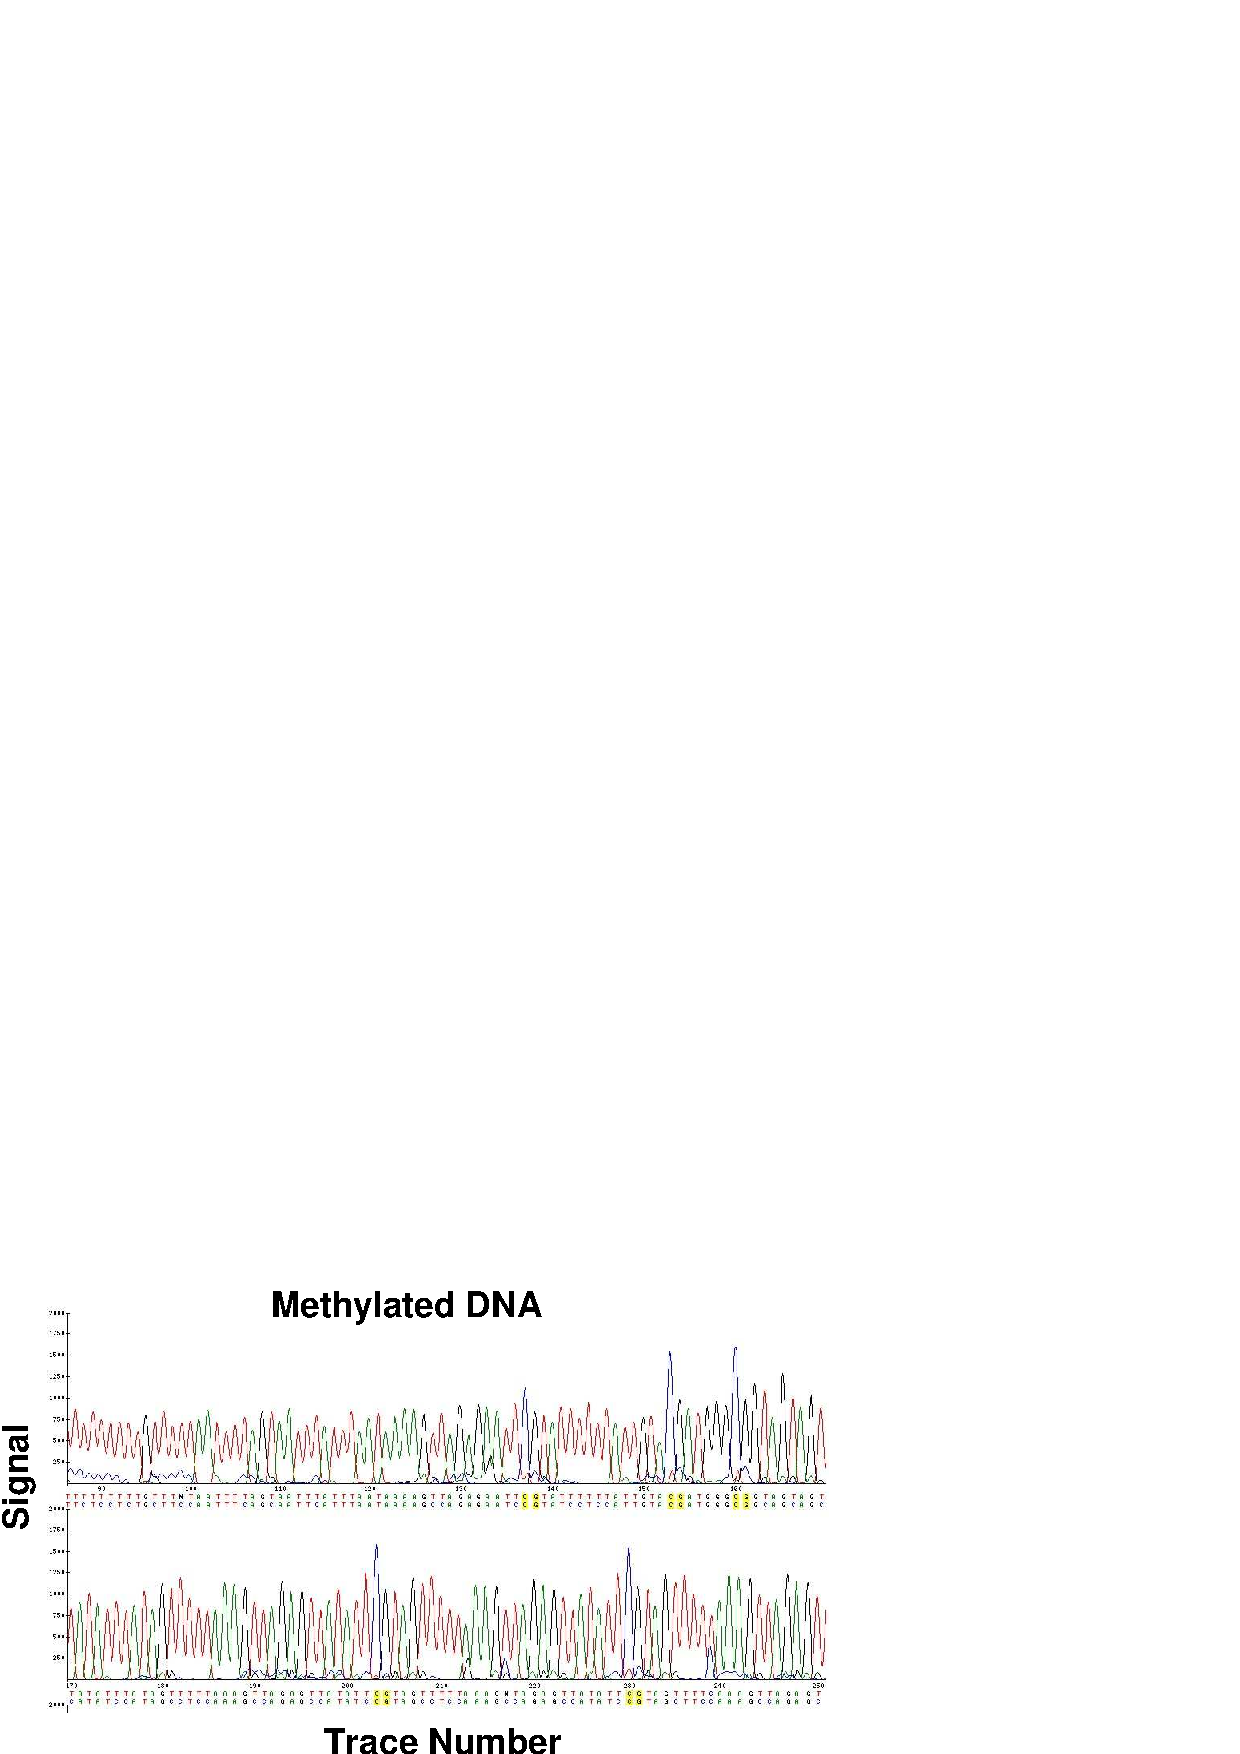
\includegraphics[width=\hsize,bb=0 0 390 230]{stamerjohanns-fig1.pdf}
    \caption{Dynamically created content of the analysis of methylated DNA. Other
    researches do not only have access to images, but to full research data.}\label{fig:stammerjohanns}
   \end{center}
\end{figure}

As a member of the Deutsche Initiative f\"ur Netzwerkinformation (DINI)
Working Groups \textsl{E-Publications}
and \textsl{Open Archives}, we are trying to establish common standards
for Scientific Institutional Repositories.

\paragraph{Collaborations}
\begin{enumerate}
    \item {\sl International University  Bremen} \\
            Prof. M. Kohlhase \\
            Extending OMDOC to PhysML, ArXiv conversion     \\
            Prof. A. Jeltsch \\
            Dynamic publishing of SMP Epigenetics Data

    \item {\sl ISN Oldenburg} \\
            Prof. E.R. Hilf \\
            Extending OMDOC to PhysML\\
            Citation Linking and Indexing

    \item {\sl DINI Working Groups} \\
            Certificate for Institutional Repositories

\end{enumerate}

%\paragraph{Publications}
\nocite{HilKohSta:copmem06,DINI06}


\shorttitle{Microelectronic Devices and Technologies}
\subsection{Microelectronic Devices and Technologies}

To continue the rate of progress in information and systems and
technologies into the next decade fundamental questions in material
science and manufacturing technology have to be answered to further
reduce the device dimension into the sub 100nm arena and increase
the complexity of integrated circuits. Novel Micro and Nano
Technologies are needed, either to overcome limitations to further
shrinking of devices and/or to implement novel electronic
hardware/services (such as large flexible displays). In parallel to
the development of novel devices, the integration into large volume
manufacturing processes and the specific problems associated to
manufacturing and quality/reliability engineering of these have to
be addressed, according to the principles of concurrent engineering.

%%% Local Variables:
%%% mode: latex
%%% TeX-master: "report"
%%% End:

\subsubsection{Electronic Devices and Nanophotonics}
\index{Knipp, Dietmar}

\paragraph{Electronic Devices and Nanophotonics group}
Dietmar Knipp (Professor), Amare Benor, Kah-Yoong Chan, Christian Haase (external PhD
student)  (PhD Student), Rahul Dewan (MSc student), Zhelio Andreev (MSc student)\\

Research of the Electronic Devices and Nanophotonics group is
focused on nano and optical technologies and their applications in
information technology and photovoltaics. The major goal of the
research is to develop the next generation of electronic and
photonic devices bridging from the micro to the nanoscale.

\paragraph{Highlights}

With the advent of micro and nano fabrication the production of nano-structured materials
in the sub 100 nm range became feasible. Such nanostructures are of interest for several
optical and photonic applications like solar cells and optical sensors.  For example, the
conversion efficiencies of thin film solar cells can be increased by nano texturing of the
cells. Due to nano texturing a larger fraction of the incoming light is scattered and
diffracted, so that the total absorption of light in the solar cell is
enhanced. Subsequently the generated photocurrent and the conversion efficiency of the
solar cell are enhanced. Despite these improvements the underlying optics in such nano
textured solar cells is not fully understood. Classical optics does not facilitate the
description of the wave propagation in such a solar cell. Maxwell's equations have to be
solved in 2D or 3D to gain insights in the optical wave propagation of such devices.  The
optics were studied by numerical simulations using a Finite Integration Technique (FIT)
and Finite Difference Time Domain (FDTD) approach. The device structure is approximated by
a solar cell with a periodic groove structure. The Figure~\ref{fig:profknipp1} (left)
shows one period of such a solar cell with a groove structure. The numerically simulated
absorption is shown in Figure~\ref{fig:profknipp1}, right.

\begin{figure}[ht]
  \begin{center}
    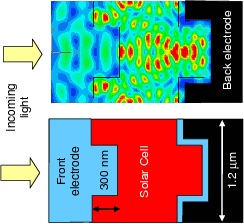
\includegraphics[width=\hsize, angle=270]{profknipp-figinfo.png}
    \mycaption{ Cross section of a slice of a nanotextured solar cell (left) and
      absorption profile in the solar cell}\label{fig:profknipp1}
   \end{center}
\end{figure}


The absorption of light in the cells is increased, due to scattering and diffraction of
light. Simulations carried out by Christian Haase show that the grooves cause an increase
of the total conversion efficiency of
10-15\%.
%The increase of the absorption is mainly observed for the infrared part of the
%optical spectrum. Based on a comparison of the experiment and the numerical
%simulation an optimized nano patterning schemes can be derived. The simulations show
%that the conversion efficiency is maximized if the height of the grooves is
%approximately equal to half of the period of the grooves.
The optical simulations were not only applied to solar cells. Numerical simulation of
metallic nanostructures shows that metallic hole arrays can be applied as optical
filters. The filter properties can be tuned by changing the diameter and the spacing of
the holes in the metal film. As the fabrication of the metallic structures is compatible
with classical micro and nanoelectronics such metallic nanostructures can be integrated in
conventional optical sensor or digital cameras. Cameras using such metallic nanostructures
would exhibit a reduced pixel cross talk and a higher spectral resolution.  In summary,
optics on the nanoscale provides a lot of new opportunities for technical
applications. Numerical simulations of the optics on the nanoscale are essential to gain a
solid understanding and optimize the device structures. In order to verify the results of
numerical simulations have to be compared to experimental results.  The research on
optics in nanostructured media is carried out in close collaboration with the research
group of Dr. H. Stiebig at the Institute of Photovoltaics, Research Center J\"ulich.

\paragraph{Collaborations}
\begin{enumerate}
\item {\sl International University Bremen} \\ Prof. Veit Wagner \\ Organic Electronics
\\ Prof. Werner Bergholz \\ Photovoltaics and Microelectronics
\item {\sl University Bremen} \\ Prof. Wolfgang Benecke \\ Microsystems Technology
\item {\sl Research Center J�lich} \\ Dr. Helmut Stiebig \\ Nanocrystalline Thin Film
  Transistors and Optics in nanostructured media
\item {\sl Bendit Innovative Interfaces} \\ J. Huyer \\ Solar Cells for mobile
  applications
\item {\sl Palo Alto Research Center} \\ Dr. R.A. Street, A.R. V�lkel. Dr. J. Northrup \\
  Organic electronics and modelling
\item {\sl Stanford University} \\ Prof. A. Salleo \\ Organic electronics

\end{enumerate}


\paragraph{Grants}
% list the running grants in 2006, if none have been received, please delete this
% subsection.
\begin{enumerate}
%\item {BMBF} ``Embedded Microsystems Bremen (EMB)''
\item Funded by {Forschungszentrum J\"ulich}, \emph{Funktionale
Kontaktschichen}, (February 2006 - January 2007)
\end{enumerate}


\paragraph{Awards, Prizes}
% list the grants you have received in 2005, if none have been received, please delete
% this subsection.
\begin{enumerate}
\item Ernst A.C. Lange Award together with Prof. W. Benecke from the Institute for
  Microsensors, -actuators, and -systems (University Bremen)
\end{enumerate}

\paragraph{Patents}
\begin{enumerate}
\item H. Stiebig, D. Knipp, J. F�lsch, Three-color sensor with a pin or nip series of
  layers, Japan, Patent number: Hei-9-535750;
\item D. Knipp, Optical sensor and integrated photonic crystal and method for producing
  the optical sensor, submitted to German patent office.
\end{enumerate}


\nocite{Knipp1, Knipp2, Knipp3, Knipp4, Knipp5, Knipp6, Knipp7, Knipp9,
Knipp10, Knipp11, Knipp13}


\subsubsection{Microelectronics}\label{ict:micro:bergholz}
\index{Bergholz, Werner}

\paragraph{Research Team}
Werner Bergholz (Professor), Thomas Dinkel (PhD student), Uwe Pagel (Technical
Assistant)\\

%%% give a very short (150 words description of your research area)
%% Hint: this can be copied from the research areas document (../masterplan/research-areas)

After 30 years of rapid advancements in microelectronics barriers are emerging for a
further device shrink and/or improvement of quality/failure rates. Our research focuses on
these ``brick walls''. These barriers are mainly related to defects, which limit yield and
reliability and the exploding cost for lithography. In addition, nanotechnology artefacts,
such as carbon nano tubes and quantum dots are getting closer to integration into
conventional microelectronic products. The specific research topics are the
\begin{myitemize}
\item Development of destruction free methods to detect defects in silicon wafers
\item Defect-related failure mechanisms and reliability test methods for microelectronic
  circuits.
\item New wafer types with functional layers to mitigate the cost explosion for
  lithography
\item Novel process control methodology to improve quality and productivity.  Unless
  solutions for the listed challenges can be identified, the rapid expansion of
  information technology will slow down within the next 5 years.  In addition, the
  following additional research topics are being addressed,
\item Investigation of defect engineering methods and efficiency detractors in Si solar
  cell technology (based on an synergy with microelectronics techniques)
\item Application of Quality Management methodology and standardisation techniques to
  nanotechnology and other non-technical areas.
\end{myitemize}
One of the more subtle limitations to further device shrink is a phenomenon known as
random telegraph signals (RTS noise) in semiconductor devices. Known and not understood
for more than 30 years, it never had particular technological importance. With devices in
the 100nm size range or below, it is gradually transforming from a laboratory curiosity to
a serious challenge in many application areas.

\begin{figure}[ht]
  \begin{center}
      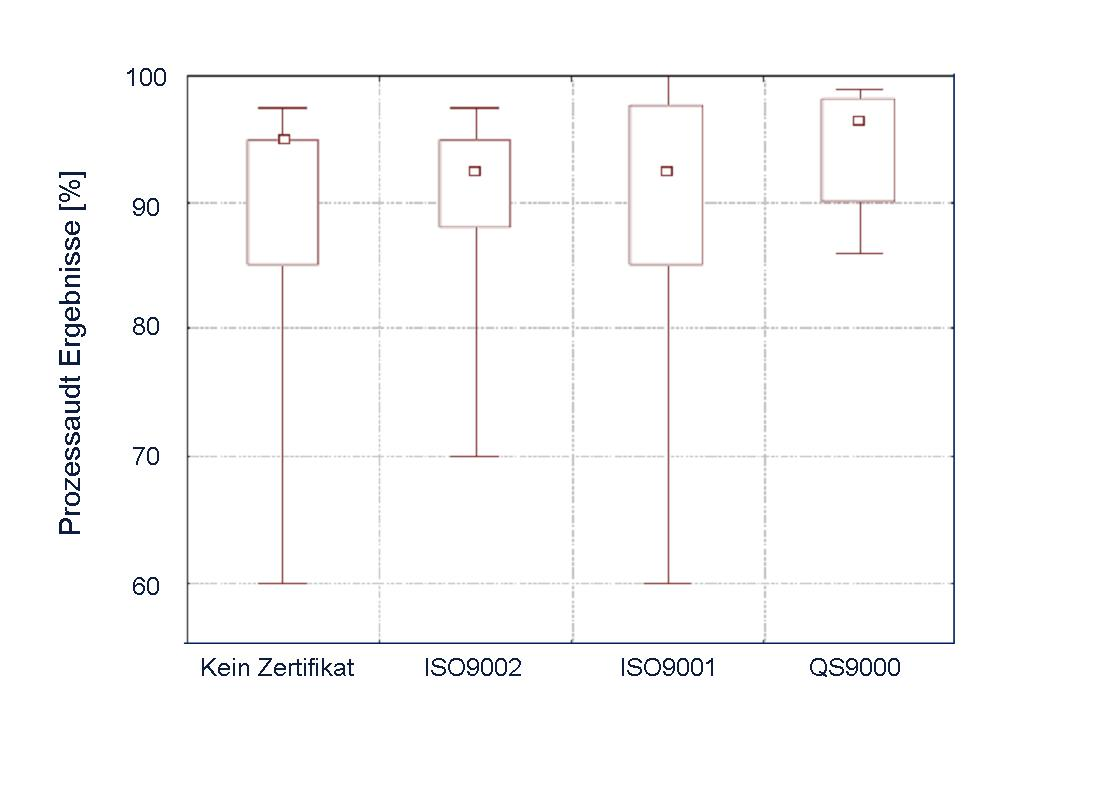
\includegraphics[width=\hsize]{EECS/bergholz-fig1}
    \mycaption{Boxplot comparison of the scores in a process-oriented audit of suppliers
      to the microelectronics industry. Suppliers which conform to the QS9000 (TS16949)
      Quality standard are clearly superior to ISO9000 certified or not certified
      companies}
    \label{fig:switching}
   \end{center}
\end{figure}

\paragraph{Highlights}

{\emph{Quality Management methodology}}: An evaluation of about 100 second party audits of
materials suppliers to the microelectronics industry has shown that a certification
according to the quality management standard TS16949 (formerly QS9000) correlates with
positive results in a process oriented audit methodology (see Fig.~\ref{fig:switching}). On
the other hand, certification according to the standard ISO9001 and ISO9002 (less
stringent than TS16949) does not guarantee a sufficient quality level, if it is compared
to the former group or companies which have no certification at all. There are also
significant differences between silicon wafer manufacturers (which have a decade long
tradition in clean room technology and high quality standards) and producers of other
materials for the Chip industry (chemicals, gases, metals etc.). Furthermore, it can be
concluded that the process oriented audit methodology is a sutiable tool to measure the
quality standard of a
supplier.\\

{\emph{Random Telegraph Signals in Si devices}}: The study of random telegraph signals in
diodes has been extended to the influence of temperture bias stress measurements
(S. Nandhavel \& W. Bergholz). After 175 degrees C (Fig.~\ref{fig:leakage}) leakage can be
observed, which is consistent with the hypothesis that metal boron pairs are the
responsible defects. Deep Level Transient Spectroscopy, radiation experiments and TEM
studies are planned to track down the defect mechanism.

{\emph{Photovoltaics industry}}: A systematic study of the open data for the process
capabilities of all major PV manufacturers has revealed an unexpected large variation in
the efficiencies and other performance indicators. It is planned to identify methods how
the process variation can be reduced by "copy intelligently" of engineering methods
developed in the microelectronics industry.

\begin{figure}[ht]
  \begin{center}
    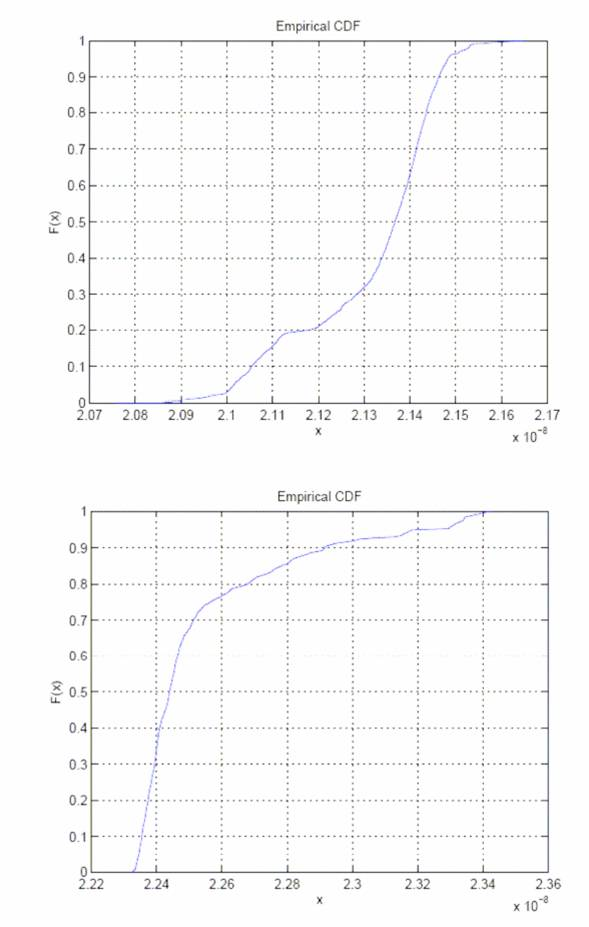
\includegraphics[width=7cm]{EECS/bergholz-fig2}
    \mycaption{After temperature bias stress of a diode there is a reversible recovery of
      the leakage currents for voltages slightly below the barrier voltage, attributed to
      diffusion pairing reactions of metal impurities, comparison of the cumulitive
      distribution function for the leakage curents before and after stress at 175 degrees
      C}
    \label{fig:leakage}
   \end{center}
\end{figure}

{\bf Outlook}: It is planned to supplement the study on audit methodology to a correlation
with a performance evaluation of the same suppliers and to extend the study to the data
gathered by a major car manufacturer in about 10 000 quality audits at suppliers to the
car industry. Objective: further refine the audit methodology and quality management
implementation methods. The Study on RTS will be extended to the investigation of methods
to reduce the effect and thus lower or remove one of the roadblocks to the
microelectronics industry. The long term goal of the PV studies is to develop efficient
defect reduction and efficiency optimization methods so as to support the goal for cost
reduction by a factor or 3 until PV becomes competive for peak power in grid
applications. The standardisation research in cooperation with DIN, DKE and SEMI is
targetted towards early anticipatory standards in emerging nanotechnology to facilitate
the transformation from lab to fab.

%\newpage
\paragraph{Organization}
\begin{enumerate}
\item Workshop: ``Silicon Wafers SEMI� Standards Workshop'', April 05 2006, Munich Trade
  Center
\item SEMI Autumn Conference: ``Conference "Bridging Semiconductor \& Related'', 08th
  Nov2006 Dresden
\end{enumerate}
\paragraph{Collaborations}
\begin{enumerate}
\item {\sl Infineon Technologies, Dresden}\\
  RTS noise phenomena
\item {\sl Infineon Technologies, Munich}\\
  Test Set up for DRAMs
\item {\sl MEMC, St. Peters, Missouri}\\
  Defect Detection in Silicon Wafers
\item {\sl Q-Cells, Thalheim}\\
  Efficiency Engineering for Silicon-based Solar Cells
\item {\sl Quintiq, S'Hertogenboch, Netherlands}\\
  Best practice Quality Management Tools for the Software Industry
\item {\sl International University Bremen}\\
  Dietmar Knipp\\
  Solar cells, low cost electronics
\item {\sl International University Bremen}\\
  Peter Ludes (SHSS), C. Schwender (JCLL)\\
  Visual mass communication
\item {\sl SEMI (Semiconductor Equipment and Materials)
    San Jose, Brussels}\\
  Bettina Weiss, Carlos Lee\\
  Semiconductor Standards Development
\item {\sl DIN, Berlin}\\
  Standardization of Nanomaterials
\item {\sl DKE, Frankfurt, Main}\\
  Standarization of Nanoelectronic Electronic Products
\end{enumerate}

\paragraph{Patents}
\begin{enumerate}
\item Patent on wafer technology, in the filing process
\end{enumerate}

\paragraph{Grants}
 \begin{enumerate}
\item Funded by Deutsches Institut f�r Normung (DIN/DKE) /
Bundesministerium f�r Wirtschaft,  \emph{Standardisierung
Nanoelektronik} (July - December 2006)
\end{enumerate}

\paragraph{Awards, Prizes}
\begin{enumerate}
\item shortlisted for the IEC centinary Award Challenge
\end{enumerate}

\newpage
%\paragraph{Publications}
%\nocite{BerWeiLee:QFD05}
%\nocite{KumWeiPagBer:ecrtnd05}
%\nocite{BaaBerg:ddf05}
\nocite{WittBerg:wbqz06}
\nocite{Berg:msinpb06}
\nocite{BergWeLee06}


%\end{description}
%\end{document}
%%% Local Variables:
%%% mode: latex
%%% TeX-master: "report"
%%% End:


\bibliographystyle{alpha}
\bibliography{profJaeger,profkohlhase,profbaumann,birk2006,henkel,profLinsen,report-pfander-2005,schoenwaelder,wallace,profantoulas,stamerjohanns,macros,cwc,report}
\end{document}
%%% Local Variables:
%%% mode: latex
%%% TeX-master: t
%%% End:
